\section{Approach}
\label{cha:approach}
% TODO: Add references to the sections and prior chapters.
% Section: OK
The following section outlines the methodological approach of this thesis. While concrete implementation details are discussed in the subsequent chapter, this section focuses on establishing the theoretical foundation that builds upon the concepts introduced in the background.
The structure of this chapter is organized according to the steps in \ref{fig:approach_overview} and begins with outlining the central objective of the thesis. There follows a set of assumptions to delimit the scope, applicability, and limitations of the proposed approach before the different steps are explained in detail.

\subsection{Central Objective - Modelling of Task Co-location}
\label{sec:problem_statement}
% Section: OK
The central objective of this work is to formally model the co-location of workflow tasks and further determine how this information can be applied during workflow execution, thereby achieving improved energy efficiency.
While this work builds upon the fundamental approach to co-locaiton of \cite{5644899} we want to specifically examine how co-location can be directly integrated into the dynamic scheduling and task mapping process, arguing that co-location and scheduling are inherently interdependent and should be addressed in a unified way. Consequently, we characterize workflow tasks before execution in order to enable contention-aware co-location decisions at runtime. The co-location in this context operates at the virtual container level, specifically focusing on virtual machines hosted on physical servers. Furthermore, we extend the question of which tasks to co-locate by the need of knowing how the performance behavior of co-located tasks can be learned and show possible means of making this knowledge accessible to resource managers.

The proposed research problem as introduced in \ref{subse:problem_motivation_description} is decomposed into six steps, seen in \ref{fig:approach_overview}. First, a data collection phase captures detailed execution metrics from scientific workflow runs. Second, this collected data undergoes structural treatment and formatting to identify relevant performance characteristics. Thirdly, the data is used to represent temporal behavior of a workflow task. This representation allows for comparison between a set of tasks to capture differences in their resource usage profiles over time and thus cluster tasks if they differ in their behavior. Step 4 arranges the collected data from step 1 in a slightly different way suitable for learning the relationship between task behavior and the resulting runtime and energy consumption. Finally, step 5 and 6 discover how the theoretical approach of step 3 can be brought into action during workflow execution and how the potential benefits of this approach can be evaluated.

% Approach Overview Figure
\begin{figure}[htbp]
    \centering
    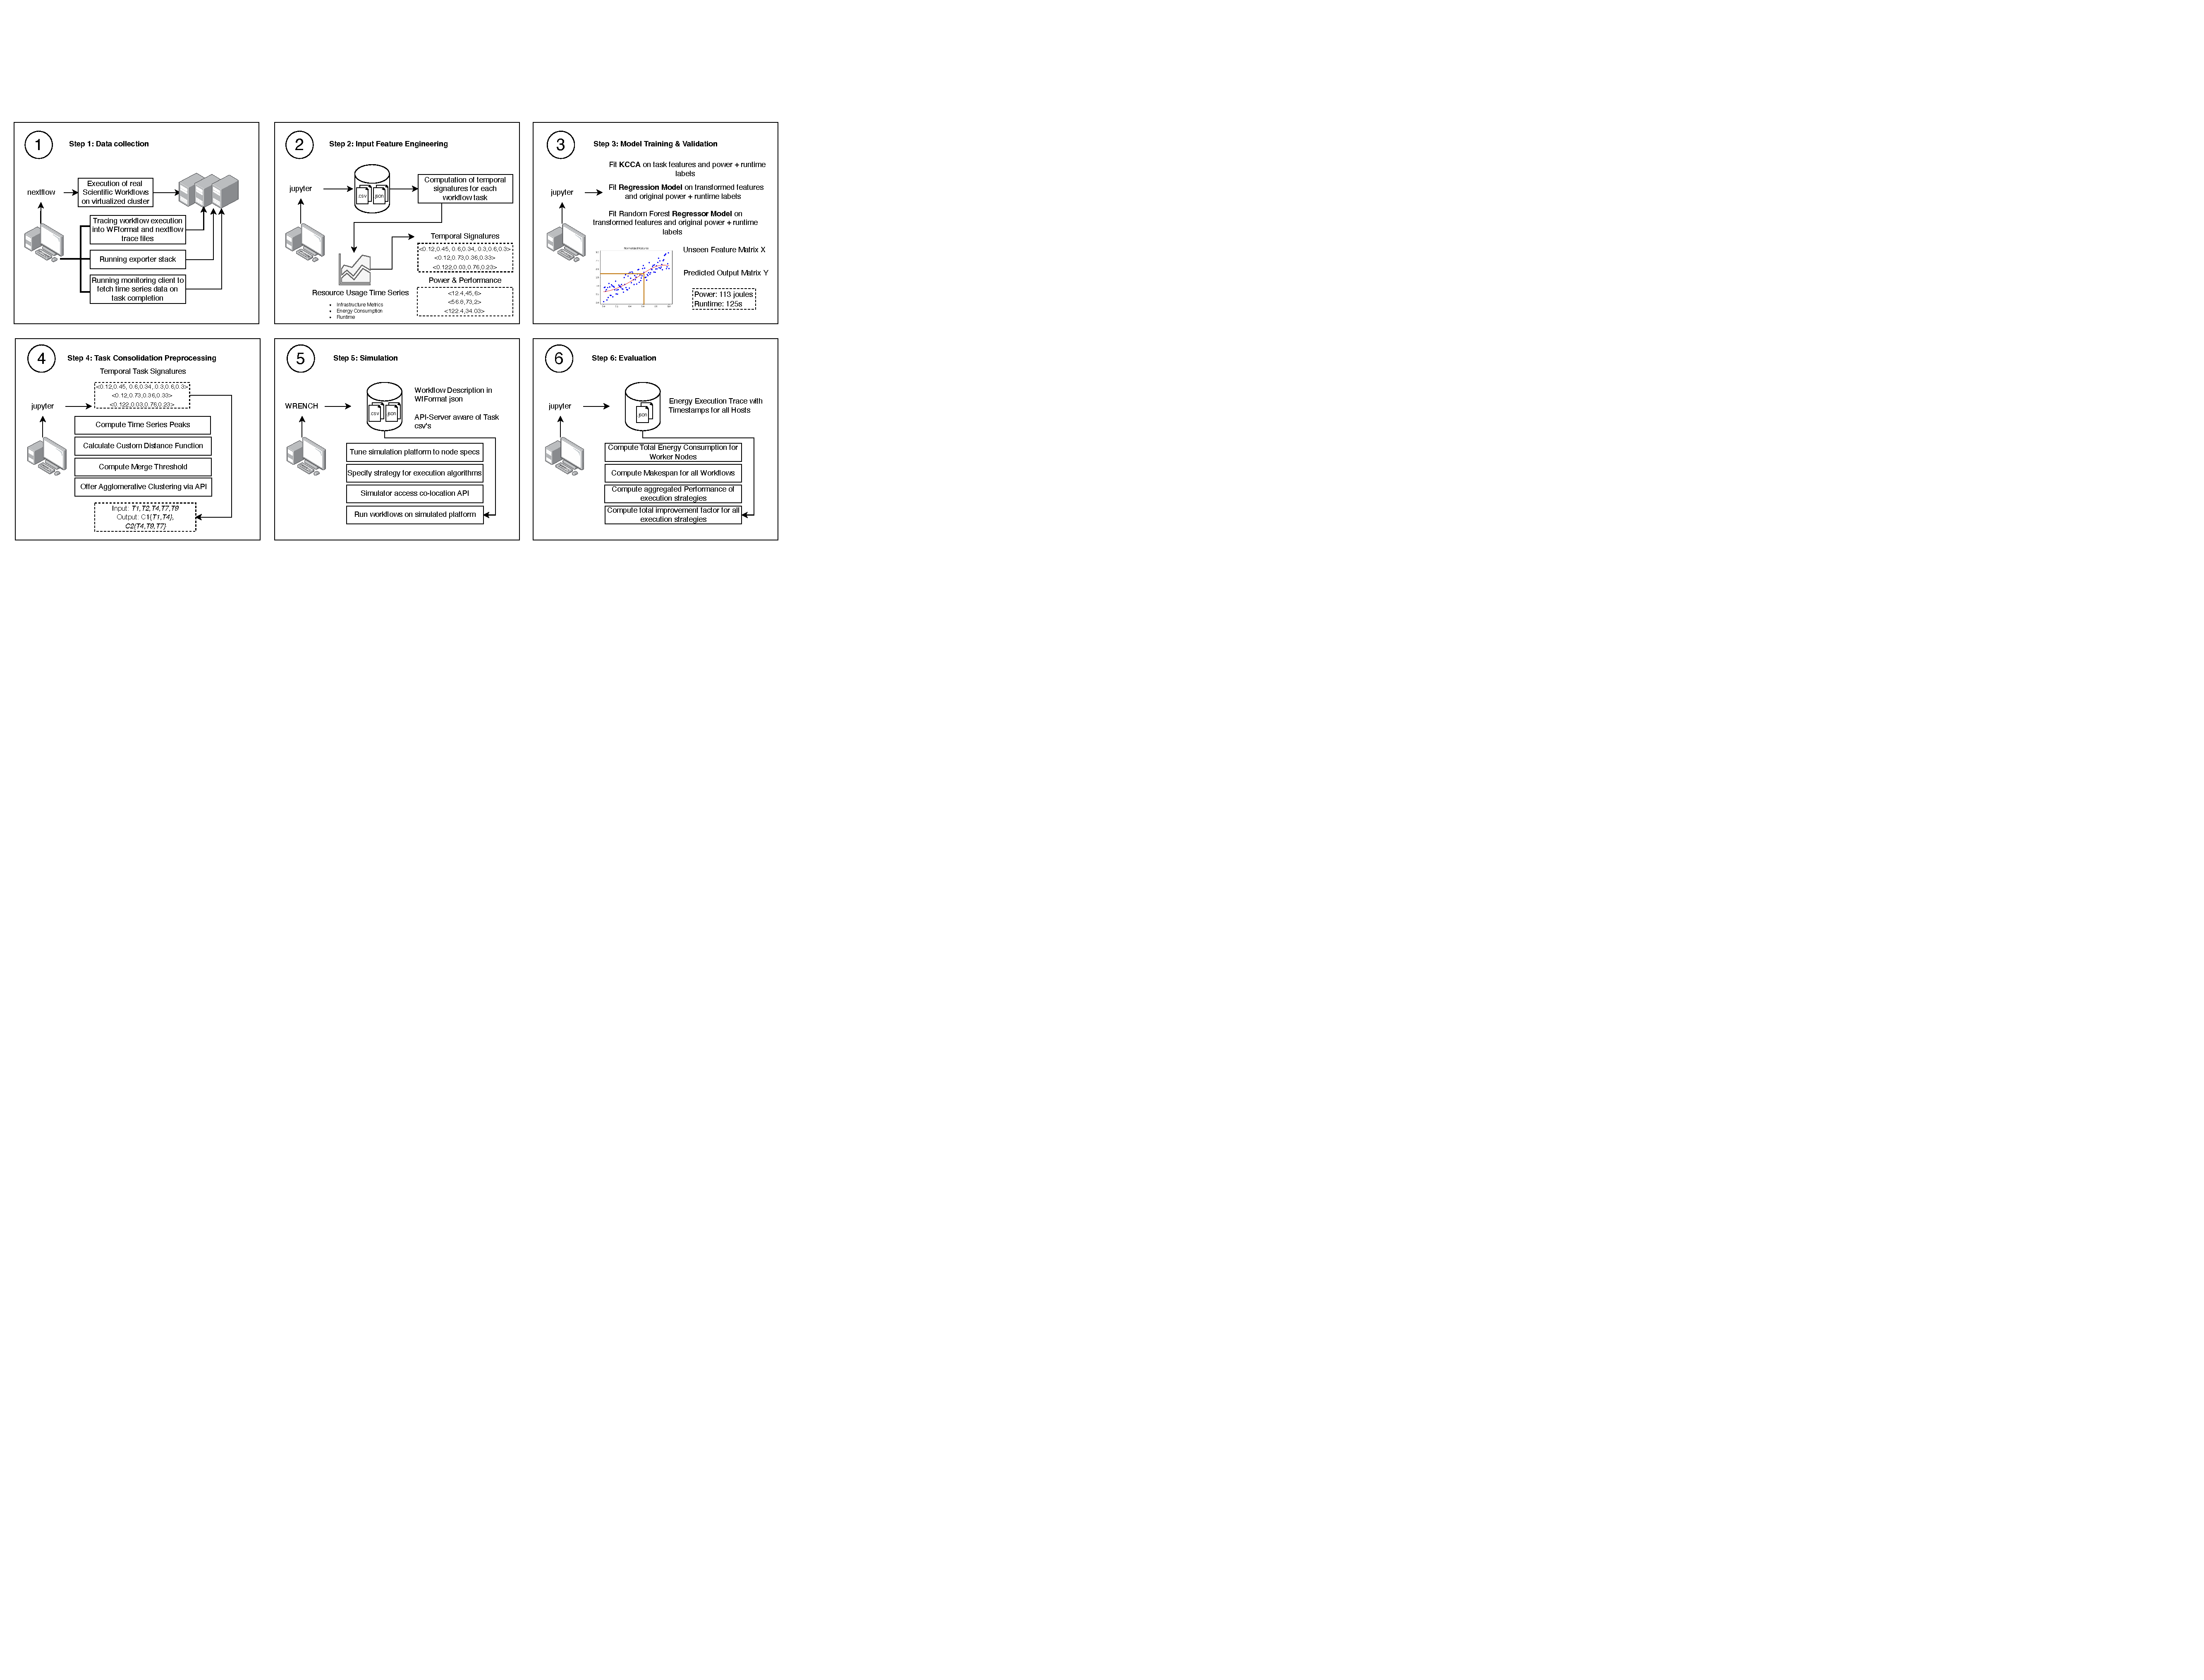
\includegraphics[width=\textwidth]{/home/nfomin3/dev/ThesisDocument/fig/04/04-overview.pdf} % Adjust the path if needed
    \caption{Overview of the approach consisting of 6 steps.}
    \label{fig:approach_overview}
\end{figure}

\subsubsection{Assumptions}
\label{sec:assumptions}
% Section: OK
To outline the scope, boundaries, and methodological constraints of this work, the following guiding assumptions were defined:

\begin{enumerate}
    \item \textbf{Monitoring Configuration Limits}:  Workflow tasks are described by 80 monitoring features. This work does not investigate the influence of monitoring data dimensionality on clustering and predictive performance.
    \item \textbf{Monitoring Data Coverage}: Short-lived tasks under one second are only partially captured or occasionally missed due to high system load and sampling intervals exceeding one second during workflow execution.
    \item \textbf{Offline Data Analysis}: The data preprocessing and predictive model fitting are performed offline after workflow execution. The co-location clustering algorithm is evaluated offline but also transformed into a suitable format for integration into the simulation environment.
    \item \textbf{Simulation Environment and Platform Equivalence}: The simulated platform is assumed to approximate the physical execution environment. It is expected that the overall behavior observed in simulation aligns with real-world execution trends.
    \item \textbf{Simulation Capabilities and Contention Modelling}: The WRENCH framework currently supports simulation of memory contention by limiting per-Host memory consumption, where exceeding the limit results in extended task execution times. Similarly, CPU contention is modeled through proportional increases in task runtime. Other low-level contention effects like cache interference, interconnect bottlenecks, or I/O contention are not modeled in this iteration. The energy model provided by SimGrid is assumed to realistically approximate energy consumption variations when tasks with differing resource usage profiles are co-located on the same virtual machine. The impact on energy efficiency is attributed to CPU utilization behavior and derived from the platform description where different load levels map to consumed energy amount.
\end{enumerate}

\subsection{Online Task Monitoring}
\label{sec:online_task_monitoring}

The online task monitoring approach builds on a hierarchical architecture that tries to capture a wide spectrum of metrics relevant to the execution of scientific workflows. The design is inspired by \cite{Bader_2022} targeting a four-layered structure consisting of the Resource Manager, Workflow, Machine, and Task layers. Each layer represents a distinct abstraction level in the workflow execution environment and provides valuable insights into different aspects of performance and resource utilization.

Starting with the Resource Manager layer a coarse-grained view related to cluster or partition status, resource allocation, and job management is provided. The Workflow layer operates on the logical workflow representation, maintaining execution progress, task dependencies, and overall runtime statistics. Below, the Machine layer captures system-level performance data such as CPU, memory, and storage utilization, as well as hardware-specific configurations. At the lowest level, the Task layer delivers fine-grained, time-resolved monitoring data, including per-task resource consumption, low-level kernel metrics, and execution traces.
\cite{Bader_2022}.

The following section provides a brief overview of the data sources and monitoring technologies that were ultimately assigned to the four layers of interest and thus selected for the approach. While the accompanying table \ref{tab:monitoring-features} presents a broader view of the different tools and data collection options that were tested we will focus only on the specific data sources that proved to be most reliable and effective within the implemented monitoring framework.

% TODO: Refine contents of the table here.
\begin{table}[htbp]
    \centering
    \setlength{\tabcolsep}{6pt} % adjust horizontal padding
    \renewcommand{\arraystretch}{1.2} % adjust vertical spacing
    \small % reduce overall text size to fit page
    \resizebox{\textwidth}{!}{
        \begin{tabular}{lccccccc}
            \toprule
            \textbf{Monitoring Features}        &
            \multicolumn{7}{c}{\textbf{Data Sources}}                                                                                                                                                                                  \\
            \cmidrule(lr){2-8}
                                                & \textbf{cAdvisor} & \textbf{ebpf-energy-exporter} & \textbf{docker-activity} & \textbf{scaphandre} & \textbf{slurm-exporter} & \textbf{process-exporter} & \textbf{cgroups-exporter} \\
            \midrule
            \multicolumn{8}{l}{\textbf{Resource Manager}}                                                                                                                                                                              \\[3pt]
            Infrastructure status               & x                 &                               &                          &                     &                         &                                                       \\
            File system status                  & x                 &                               &                          &                     &                         &                           &                           \\
            Running workflows                   & x                 &                               &                          &                     &                         &                           &                           \\
            \midrule
            \multicolumn{8}{l}{\textbf{Workflow}}                                                                                                                                                                                      \\[3pt]
            Status                              & x                 & x                             &                          &                     &                         &                           &                           \\
            Workflow specification              &                   & x                             &                          &                     &                         &                           &                           \\
            Graphical representation            &                   & x                             &                          &                     &                         &                           &                           \\
            Workflow ID                         & x                 & x                             &                          &                     &                         &                           &                           \\
            Execution report                    &                   & x                             &                          &                     &                         &                           &                           \\
            Previous executions                 &                   & x                             &                          &                     &                         &                           &                           \\
            \midrule
            \multicolumn{8}{l}{\textbf{Machine}}                                                                                                                                                                                       \\[3pt]
            Status                              &                   &                               & x                        & x                   &                         &                           &                           \\
            Machine type                        &                   &                               & x                        & x                   &                         &                           &                           \\
            Hardware specification              &                   &                               & x                        & x                   &                         &                           &                           \\
            Available resources                 &                   &                               & x                        & x                   &                         &                           &                           \\
            Used resources                      &                   &                               & x                        & x                   &                         &                           &                           \\
            \midrule
            \multicolumn{8}{l}{\textbf{Task}}                                                                                                                                                                                          \\[3pt]
            Task status                         &                   &                               &                          & x                   &                         &                           &                           \\
            Requested resources                 &                   &                               &                          & x                   &                         &                           &                           \\
            Consumed resources                  &                   &                               &                          & x                   &                         &                           &                           \\
            Resource consumption for code parts &                   &                               &                          & x                   &                         &                           &                           \\
            Task ID                             &                   &                               &                          & x                   &                         &                           &                           \\
            Application logs                    &                   &                               &                          & x                   &                         &                           &                           \\
            Task duration                       &                   &                               &                          & x                   &                         &                           &                           \\
            Low-level task metrics              &                   &                               &                          & x                   &                         &                           &                           \\
            Fault diagnosis                     &                   &                               &                          & x                   &                         &                           &                           \\
            \bottomrule
        \end{tabular}
    }
    \caption{Technologies and their capabilities evaluated against a 4-layered Monitoring Framework for Scientific Workflows.}
    \label{tab:monitoring-features}
\end{table}

To enable access to detailed performance metric in time-series format we chose to use Prometheus as the central time-series database. As shown in the \ref{tab:monitoring-features}, we consequently focused on tools that are interoperable with Prometheus as data exporters and examine their level of operation in layered monitoring framework.
Due to different reasons certain exporters that are listed in \ref{tab:monitoring-features} were excluded from further use. The Slurm exporter, a custom implementation, was originally intended to retrieve job-to-process mappings from the resource manager. However, equivalent information could also be obtained directly from the workflow engines tracing mechanism, and because the programmatic interaciton with Slurm's daemons introduced considerable overhead, the exporter was not used in later stages. The process exporter was also omitted due to difficulties in collecting and aggregating all process IDs associated with a single container. In many cases, only the initial shell process of a workflow task was captured, while its spawned subprocesses remained untracked.
Scaphandre, despite appearing promising at first, showed limited compatibility with different hardware architectures. The tool also struggled to capture short-lived workflow tasks leading to incomplete datasets. Docker-Activity imposed the same limitations as scaphandre.

The most consistent and comprehensive results were achieved using cAdvisor and a custom fork of the DEEP-mon system, presented in \cite{8425477}. These two tools demonstrated the best stability and coverage across different task durations and resource types and were therefore selected for the final monitoring setup.

The following table presents the final selection of data sources that were retained for the monitoring setup, along with the specific metrics enabled for each source.

% Table with Tool Overview and metrics
\begin{table}[htbp]
    \centering
    \setlength{\tabcolsep}{6pt}
    \renewcommand{\arraystretch}{1.2}
    \small
    \caption{Preliminary simulation results for a subset of workflows showing the overall improvement for both runtime and energy consumption compared to the average of 2 naive baselines without co-location.}
    \label{tab:workflow_results}
    % \resizebox{\textwidth}{!}{%
    \resizebox{\textwidth}{0.46\textheight}{%
        \begin{tabular}{
            >{\raggedright\arraybackslash}p{2.7cm}
            >{\raggedright\arraybackslash}p{3.3cm}
            >{\raggedright\arraybackslash}p{7cm}
            >{\raggedright\arraybackslash}p{2.7cm}
            }
            \toprule
            \textbf{Software Tool} & \textbf{Primary Focus}                  & \textbf{Used Metrics}                               & \textbf{Comment}                                                           \\
            \midrule
            nextflow               & Scientific Workflow Engine              & trace file summary                                  & Used for WfFormat generation and matching containers to nextflow processes \\
            \midrule
            cAdvisor               & Container Performance Monitor           & \makecell[l]{container\_memory\_working\_set\_bytes                                                                              \\container\_memory\_usage\_bytes\\container\_memory\_rss\\container\_fs\_reads\_bytes\_total\\container\_fs\_writes\_bytes\_total\\container\_fs\_io\_current} & 11191 \\
            \midrule
            ebpf-monitor           & Container Energy \& Performance Monitor & \makecell[l]{container\_memory\_working\_set\_bytes                                                                              \\container\_memory\_usage\_bytes\\container\_memory\_rss\\container\_fs\_reads\_bytes\_total\\container\_fs\_writes\_bytes\_total\\container\_fs\_io\_current\\container\_mem\_rss\\container\_mem\_pss\\container\_mem\_uss\\container\_kb\_r\\container\_kb\_w\\container\_num\_reads\\container\_disk\_avg\_lat\\container\_num\_writes\\container\_cycles\\container\_cpu\_usage\\container\_cache\_misses\\container\_cache\_refs\\container\_weighted\_cycles\\container\_power\\container\_instruction\_retired} & 39216.4 \\
            \bottomrule
        \end{tabular}%
    }
\end{table}

% Description of cadvisor, ebpf-energy-monitor
cAdvisor is an open-source daemon for monitoring resource usage and performance of containers. It continuously discovers containers via Linux cgroups under the path /sys/fs/cgroup. Once started, cAdvisor subscribes to create/delete events in the cgroup filesystem, converts them to internal add/remove events, and configures per-container handlers. Metrics originate from machine-level facts parsed from /proc and /sys directories and most prominently container and process usage collected at cgroup boundaries. In practice, cAdvisor provides low-overhead, per-container telemetry.%\cite{Tol}.

DEEP-Mon is a per-thread power attribution method to translate coarse-grained hardware power measurements into fine-grained, thread-level energy estimates by exploiting hardware performance counters. The Intel RAPL interface provides power readings per processor package or core, but it cannot distinguish how much of that energy was consumed by each thread. DEEP-Mon bridges this gap by observing how actively each thread uses the processor during each sampling interval. It does so by monitoring the number of unhalted core cycles—a counter that measures how long a core spends executing instructions rather than idling. Since power consumption correlates almost linearly with unhalted core cycles, the fraction of total cycles attributed to each thread provides a reasonable proxy for its share of energy usage. DEEP-mon first computes the weighted cycles for each thread—combining its active cycles when alone with its proportionally reduced cycles when co-running. These weighted cycles determine how much of the total core-level RAPL energy should be assigned to that thread. The final per-thread power estimate is then derived by distributing the total measured power of each socket proportionally to the weighted cycle counts of all threads running on that socket. This approach allows DEEP-mon to infer realistic thread-level power usage even in systems with simultaneous multithreading and time-shared workloads, without modifying the scheduler or requiring any application-specific instrumentation. The DEEP-mon tool was modified in this work to export container-level metrics directly to Prometheus.

Based on this identification of relevant metrics and the according technologies, we now introduce the monitoring algorithm built on top of the selected exporter stack and the resulting overview of the needed components. It outlines how these components were combined to realize the monitoring logic in this work, while the technical implementation details are described in \ref{cha:implementation}.

\begin{figure}[htbp]
    \centering
    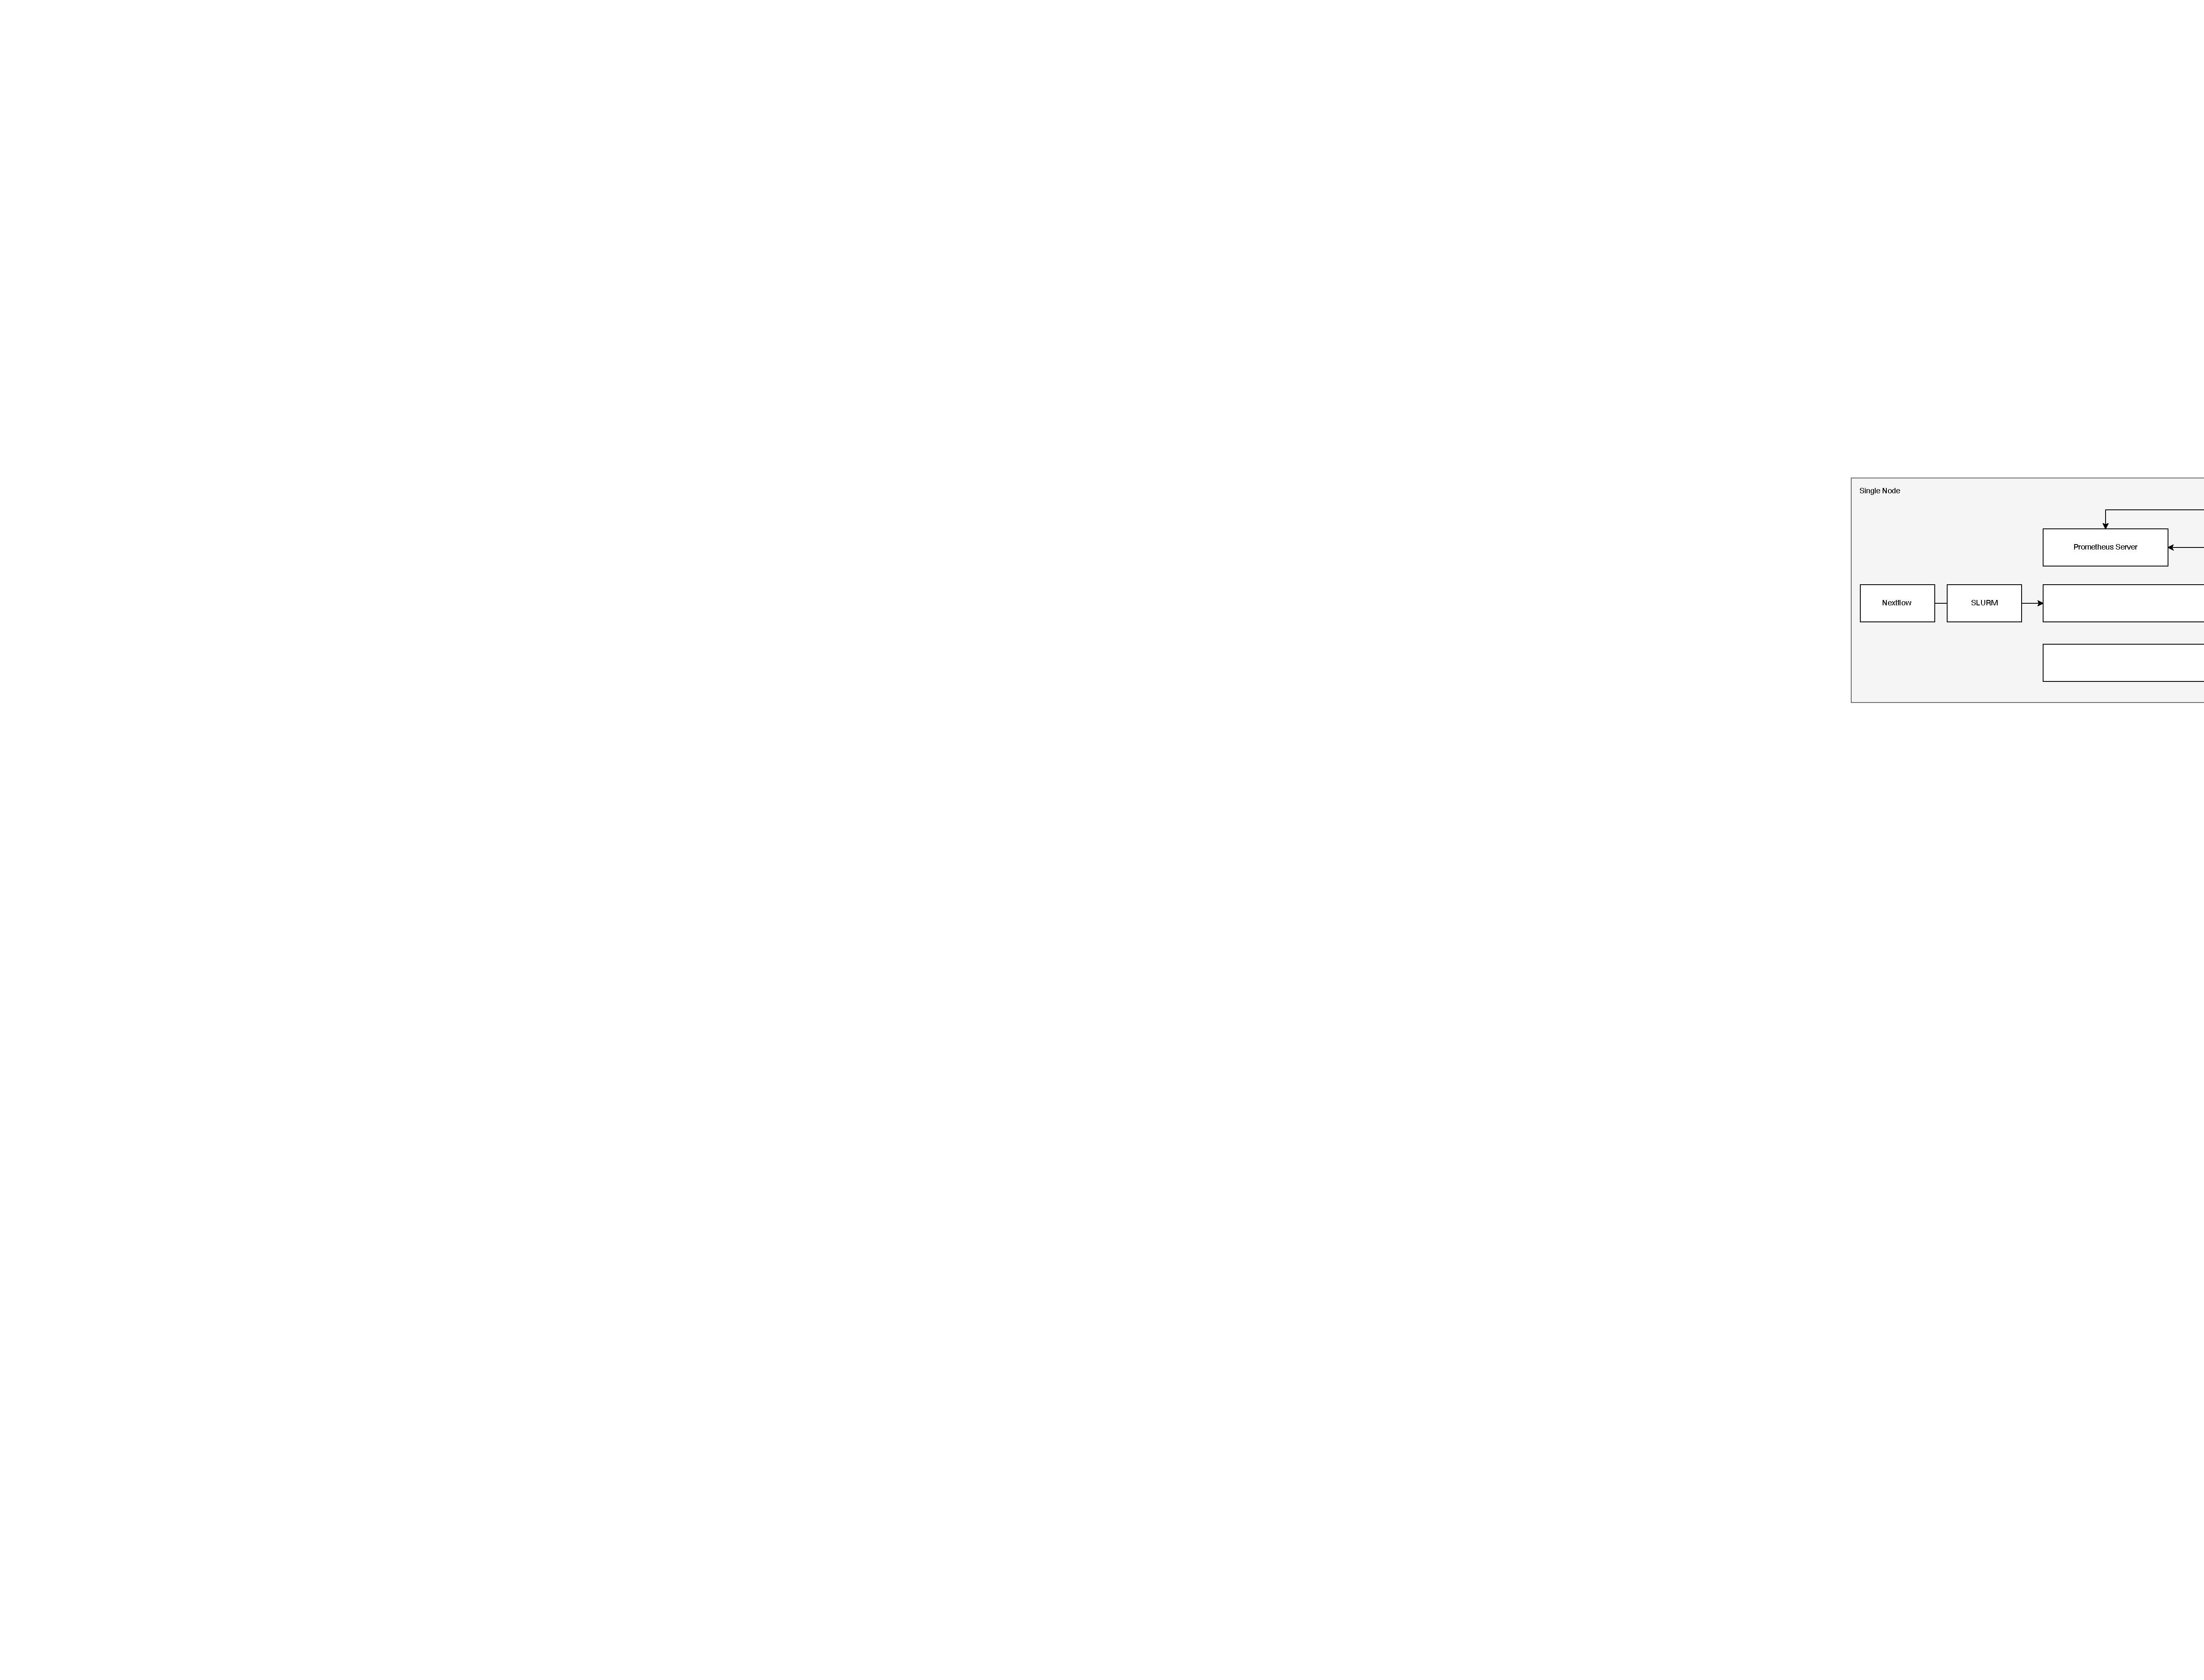
\includegraphics[width=\textwidth]{/home/nfomin3/dev/ThesisDocument/fig/04/04-monitoring.pdf} % Adjust the path if needed
    \caption{The monitoring client alongside the needed system components.}
    \label{fig:monitoring_client}
\end{figure}

\ref{fig:monitoring_client} and \ref{alg:monitoring} show the behavior of the monitoring client. The event listener continuously observes container lifecycle events—such as start and termination—emitted by the runtime environment. Once an event is detected, the data query interface dynamically formulates PromQL queries based on the configuration and metadata of the affected container. These queries are sent to Prometheus to retrieve fine-grained time-series data. The retrieved raw metrics are then passed to the aggregation module, which aligns and consolidates them into a unified record per container.

\begin{algorithm}[H]
    \caption{Event-Driven Monitoring and Metric Aggregation Framework}
    \label{alg:monitoring}
    \KwIn{Configuration $C$ defining monitoring targets}
    \KwOut{Aggregated container-level time-series metrics for each Nextflow process}

    \BlankLine
    initialize\_monitoring(C)\\
    init\_event\_listener()\\
    \While{true}{
        event $\gets$ wait\_for\_container\_event()\\
        meta $\gets$ extract\_metadata(event)\\
        \If{event.type = START}{
            register\_process(meta.id, meta.workflow\_label)
        }
        \If{event.type = TERMINATE}{
            metrics $\gets$ \{\}\\
            \ForEach{target $\in$ C.targets}{
                query $\gets$ build\_promql(target, meta.id, meta.time\_window)\\
                metrics[target] $\gets$ execute\_prometheus\_query(query)
            }
            data $\gets$ aggregate(metrics, meta.workflow\_label)\\
            store(data)
        }
    }
\end{algorithm}

% Algorithm Description
The design introduced in \ref{alg:monitoring} reduces monitoring overhead and ensures that only relevant data is collected when workflow tasks execute. When a container start event is received, the client extracts metadata such as container ID, associated workflow label, and start timestamp, then registers the process in an internal mapping to maintain correspondence between container identifiers and workflow tasks. Upon receiving a termination event, the client triggers a targeted data collection phase. The monitoring client allows for dynamic configuration of the metrics mentioned in \ref{tab:monitoring-features}, enabling data analysis specifically scoped to the user's needs.

\subsection{Modelling the Co-location of Task Behavior based on Time-Series}
\label{sec:data_analysis}
This section covers step 2, 3 and 4 seen in \ref{fig:approach_overview} and describes how the collected monitoring data is processed to derive task behavior representations suitable for co-location clustering and predictive modeling.

\paragraph{General Preprocessing of Raw Time-Series Data}
\label{sec:data_preprocessing_general}

The collected monitoring data consists of raw time-series files in CSV format. Therefore, an initial step of pre-processing is necessary.

% Paragraph about generic preprocessing of raw data
\begin{enumerate}
    \item Parsing of raw time-series CSV files.
    \item Alignment of timestamps across different sources.
    \item Merging of per-task data into unified records.
    \item Matching Entities between execution layer and workflow layer
\end{enumerate}

% TODO: Maybe visualize and explain easier.
During workflow execution, diverse monitoring tools and system components produce data at different abstraction levels.
We use container lifecycle records, which provide information on task identifiers, container names, process hashes, and working directories of the workflow task. These files serve as the primary link between workflow-level entities and low-level cotnainer monitoring data. Each monitoring source is traversed recursively to locate and load the associated time-series data. These data files are organized hierarchically under source-specific directories. To facilitate task-level analysis, these aggregated time-series datasets need to be split into per-task CSV files.
We attach the correct working directory to every container trace and extract task names and their corresponding working directories. These entries are matched against container-level records from the monitoring data to identify which monitored container corresponds to which task in the workflow.

\subsubsection{Task Clustering for Contention-Aware Consolidation}
\label{sec:task_clustering}

After concluding the initial preprocessing of the raw time-series data we proceed with further refinement of the data according to the needs of performing task clustering.

\paragraph{Preprocessing Raw Time-Series Data for Task-Clustering}
\label{sec:data_preprocessing_predictive}

We apply the following two main steps prior to the clustering algorithm.

\begin{enumerate}
    \item \textbf{Peak-pattern construction}. For every task and monitored workload type, we first derive a peak time series: the raw per-second resource signal is resampled into three-second buckets and the maximum per bucket is retained. When two peak series must be compared, we truncate both to the shorter length so that correlation is computed on aligned vectors without padding artifacts.
    \item \textbf{Computing Workload-type affinity}. Different resource domains interfere to different degrees such as CPU vs CPU peaks are typically more contentious than CPU vs file I/O. We encode this by computing an affinity score between workload types which is described in \ref{sec:measuring_resource_contention}. High affinity means higher potential interference when peaks align; low affinity reflects benign coexistence.
\end{enumerate}

% Workload experiments
\paragraph{Measuring Resource Interference of Co-located Benchmarks}
\label{sec:measuring_resource_contention}

The measurement of resource contention follows a two-stage protocol that first establishes isolated baselines for each workload class and then repeats the same workloads under controlled co-location. In the baseline stage, CPU-bound, memory-bound, and file-I/O-bound benchmark containers are executed one at a time on pinned logical CPUs. Each run records a start and finish timestamp at microsecond resolution. In parallel, Deep-Mon is used to record the power time series for each container. After a run finishes, the power streams of the containers are retained, aligned to the containers lifetime, and summarized to a representative mean value.
After isolated benchmark execution we replay the same benchmarks in pairs to expose interference effects by CPU pinning. The experiment binds pairs of benchmarks to siblings on the same physical core to amplify shared-core effects. Each co-located container is measured in exactly the same way as in isolation, producing a matched set of durations and power summaries.

Table \ref{tab:synthetic-benchmarks} shows the benchmarks specifications used to generate the workloads.

% Table for the experiment design

\begin{table}[htbp]
    \centering
    \caption{Summary of Synthetic Benchmarks Used in Evaluation}
    \label{tab:synthetic-benchmarks}
    \begin{tabular}{@{}lcccc@{}}
        \toprule
        \textbf{Benchmark Label}                                                                                                                          & \textbf{Image / Version} & \textbf{Execution Command} & \textbf{Behavior Type} & \textbf{Comments} \\
        \midrule

        \textbf{CPU}                                                                                                                                      &
        \texttt{stress-ng-cpu:latest}                                                                                                                     &
        \texttt{stress-ng --cpu 1 --cpu-method matrixprod --cpu-ops 100000 --metrics-brief}                                                               &
        CPU-bound, matrix computation kernel.                                                                                                             &
        Used to emulate high arithmetic intensity workloads.                                                                                                                                                                                                   \\

        \textbf{Memory (VM)}                                                                                                                              &
        \texttt{stress-ng-mem-vm:latest}                                                                                                                  &
        \texttt{stress-ng --vm 1 --vm-bytes 18G --vm-ops 1000 --metrics-brief}                                                                            &
        Memory-bound workload.                                                                                                                            &
        Tests VM allocation, memory contention, and NUMA effects.                                                                                                                                                                                              \\

        \textbf{File I/O}                                                                                                                                 &
        \texttt{fio:latest}                                                                                                                               &
        \texttt{fio --name seqread --rw read --bs 1M --size 18G --numjobs 1 --readonly=1 --direct=1 --iodepth=32 --ioengine=io\_uring --group\_reporting} &
        I/O-intensive sequential read.                                                                                                                    &
        Evaluates disk and I/O scheduling performance.                                                                                                                                                                                                         \\
        \bottomrule
    \end{tabular}
\end{table}

% Notation for the experiments.
In order to derive a workload affinity from the contention experiments we define contention effects to occur when co-located workloads exceed their duration and power consumption compared to their isolated measurements.
\[
    \textbf{Isolated and Co-located Metrics.}
\]

For each workload \( i \in \{1,2\} \), let
\[
    t_i^{(iso)}, \; t_i^{(coloc)} \quad \text{denote the isolated and co-located runtimes,}
\]
\[
    P_i^{(iso)}, \; P_i^{(coloc)} \quad \text{denote the average isolated and co-located power consumption.}
\]

\[
    \textbf{Per-workload Slowdown Factors.}
\]

For each workload \( i \in \{1, 2\} \), let
\[
    t_i^{(iso)}, \; t_i^{(coloc)} \quad \text{denote isolated and co-located runtimes,}
\]
\[
    P_i^{(iso)}, \; P_i^{(coloc)} \quad \text{denote isolated and co-located average power consumptions.}
\]

The per-workload slowdowns are defined as
\[
    S_i^{(t)} = \frac{t_i^{(coloc)}}{t_i^{(iso)}},
    \qquad
    S_i^{(P)} = 1 + \log\!\left(
    \max\!\left( \frac{P_i^{(coloc)}}{P_i^{(iso)}}, 1 \right)
    \right),
\]
ensuring that both runtime and power slowdowns are
non-negative and at least one in value.

The mean slowdowns across the workload pair are
\[
    \bar{S}^{(t)} = \frac{S_1^{(t)} + S_2^{(t)}}{2},
    \qquad
    \bar{S}^{(P)} = \frac{S_1^{(P)} + S_2^{(P)}}{2}.
\]

A weighted average combines both effects:
\[
    \bar{S} =
    \alpha\, \bar{S}^{(t)} + (1 - \alpha)\, \bar{S}^{(P)},
    \quad \text{with } \alpha \in [0,1],
\]
where higher \(\alpha\) emphasizes runtime effects,
and lower \(\alpha\) gives more weight to power efficiency.

The final combined slowdown factor is
\[
    \bar{S}_{\text{final}} = \max(1, \bar{S}),
\]
guaranteeing that co-location never yields an apparent
speedup (values \(\ge 1\) indicate slowdown).

\[
    \textbf{Affinity Score.}
\]

The affinity score \(A\) quantifies the degree of
interference between two co-located workloads.

First, compute pairwise affinity ratios:
\[
    A^{(t)} =
    \frac{t_1^{(coloc)} + t_2^{(coloc)}}
    {t_1^{(iso)} + t_2^{(iso)}},
    \qquad
    A^{(P)} =
    1 + \log\!\left(
    \max\!\left(
    \frac{P_1^{(coloc)} + P_2^{(coloc)}}
    {P_1^{(iso)} + P_2^{(iso)}},
    1
    \right)
    \right).
\]

A weighted average combines both effects:
\[
    A_{\text{raw}} =
    \alpha\, A^{(t)} + (1 - \alpha)\, A^{(P)},
    \qquad A_{\text{raw}} \ge 1.
\]

The normalized affinity score is then:
\[
    A =
    \frac{1 - \frac{1}{A_{\text{raw}}}}{\beta},
    \qquad A \in [0, 1],
\]
where \(\beta > 0\) controls scaling sensitivity.
Values of $A \approx 0$ indicate minimal interference,
while \(A \to 1\) signifies strong co-location interference.

% TODO: Put into evaluation.
\begin{table}[H]
    \centering
    \caption{Affinity scores between workload types indicating co-location compatibility.}
    \label{tab:affinity_scores}
    \begin{tabularx}{\textwidth}{l l c X}
        \toprule
        \textbf{Workload 1} & \textbf{Workload 2} & \textbf{Affinity Score} & \textbf{Comment}                                                                              \\
        \midrule
        mem                 & cpu                 & 0.543                   & Moderate compatibility; memory and CPU workloads can share resources with limited contention. \\
        mem                 & fileio              & 0.148                   & Very low compatibility; strong interference due to I/O and memory bandwidth pressure.         \\
        fileio              & cpu                 & 0.223                   & Low compatibility; CPU workloads cause contention for shared I/O buffers.                     \\
        cpu                 & cpu                 & 0.444                   & Medium self-affinity; CPU-bound tasks compete for cores but remain schedulable.               \\
        mem                 & mem                 & 0.514                   & Moderate self-affinity; memory contention manageable under shared caching.                    \\
        fileio              & fileio              & 0.346                   & Limited self-affinity; file I/O contention degrades throughput under co-location.             \\
        \bottomrule
    \end{tabularx}
\end{table}

\paragraph{Algorithmic Approach to Task Consolidation}
Consolidation is formulated as a clustering problem with an important modification: rather than grouping tasks that are similar, the goal is to cluster tasks with complementary resource usage patterns to minimize contention during co-location. Building on the previously established notion of affinity—which quantifies how strongly workloads interfere when sharing resources—the clustering process now incorporates this measure directly into its distance metric. The task task distance increases when two tasks exert pressure on the same resources simultaneously, indicating potential contention, and decreases when their resource usage peaks complement one another.

Algorithm \ref{alg:task_distance_clustering} summarizes the main stages of the task consolidation procedure used in this work. The approach begins by computing pairwise similarities between task signatures, where each signature represents a multi-dimensional profile of resource usage over time. The similarity computation incorporates resource affinity weights derived from the contention experiments. This yields a resource-aware similarity matrix that reflects how well tasks can coexist on the same node without interference.
Next, a percentile-based threshold is applied to the similarity matrix. This adaptive rule determines when clustering should stop by selecting only the most suitable task pairs according to the defined percentile. In this way, the algorithm avoids arbitrary distance cutoffs and instead adapts to the underlying distribution of similarity values.
Finally, agglomerative clustering is performed using a specified linkage criterion, such as average or complete linkage, to iteratively merge tasks into clusters.

% Algorithm for Task Consolidation in ShaReComp
\begin{algorithm}[H]
    \caption{ShaReComp - Task Consolidation Algorithm}
    \label{alg:task_distance_clustering}
    \SetKwFunction{Sim}{compute\_similarity}
    \SetKwFunction{Thresh}{percentile\_threshold}
    \SetKwFunction{Merge}{agglomerative\_merge}

    \KwIn{task signatures $\mathrm{sig}$, affinity weights $w$, percentile $\tau$, linkage}
    \KwOut{clusters $\mathcal{C}$}

    $S \gets$ \Sim($\mathrm{sig}$, $w$) \tcp*[r]{resource-aware similarity}
    $\theta \gets$ \Thresh($S$, $\tau$) \tcp*[r]{percentile-based stopping rule}
    $\mathcal{C} \gets$ \Merge($S$, $\theta$, linkage) \tcp*[r]{agglomerative clustering}

    \textbf{return } $\mathcal{C}$
\end{algorithm}

With \ref{alg:task_distance_clustering} we introduce the ShaReComp algorithm. ShaReComp stands for share resources for computation and summarizes the goal of the method: to group tasks that can share resources effectively when co-located.
The key steps of the algorithm are as follows:

\begin{enumerate}
    \item Anti-similarity distance. For any pair of tasks i,j, we iterate over their workload types and use two factors: (i) the affinity between the two types; (ii) the correlation between their corresponding peak series computed twice, once per type, to capture both sides of the pairing. We then aggregate these terms so that highly correlated peaks in high-affinity domains increase the distance, whereas low or negative correlations in low-affinity pairs decrease it. The result is a symmetric task distance matrix whose off-diagonal entries quantify how bad it would be to co-locate the two tasks, and whose diagonals are zero by definition.

          % Notation for the distance formula
          \[
              \textbf{Inter-Task Distance and Resource Correlation Model}
          \]

          To quantify the similarity and potential contention between two workloads
          \( i \) and \( j \), we define a composite distance measure
          that integrates both resource affinity and correlation of peak usage.
          Each workload utilizes a set of resources
          \( R = \{ \text{CPU}, \text{Memory}, \text{Disk}\} \),
          yielding in total ten pairwise combinations of resource types across two tasks.
          The distance term combines the precomputed affinity score with the
          correlation of peak resource intensities.

          \[
              D_{i,j}
              = \sum_{R_1, R_2}
              \Bigl(
              (\mathrm{aff\text{-}score}(R_1^i, R_2^j))
              \cdot
              \mathrm{Corr}(\mathrm{peak}\,R_1^i, \mathrm{peak}\,R_1^j)
              \cdot
              \mathrm{Corr}(\mathrm{peak}\,R_2^i, \mathrm{peak}\,R_2^j)
              \Bigr)
              \tag{1}
          \]

          where:
          \begin{align}
              R_1^i, R_2^j & \; \text{denote resource types of workloads } i \text{ and } j,                           \\[4pt]
              \mathrm{Corr}(\mathrm{peak}\,R_1^i, \mathrm{peak}\,R_1^j)
                           & \; \text{is the Pearson correlation between the peak usages of resource } R_1,            \\[4pt]
              \mathrm{aff\text{-}score}(R_1^i, R_2^j)
                           & \in [0, 1] \text{ measures the degree of interference between } R_1^i \text{ and } R_2^j.
          \end{align}

          \[
              \textbf{Interpretation}
          \]

          The intuition behind this distance metric is to
          \emph{promote dissimilar task pairings} for co-location.
          If two workloads exhibit highly correlated peak usage on the same resources,
          their corresponding correlation terms will be large,
          thus increasing \( D_{i,j} \) and discouraging their co-location.
          Conversely, tasks with uncorrelated or complementary resource peaks
          yield smaller distance values and are therefore more suitable to merge.

          The affinity score modulates this behavior:
          smaller values of \( \mathrm{aff\text{-}score} \)
          indicate lower interference between resource pairs,
          which can offset strong peak correlations.

          Finally, clustering proceeds by iteratively merging task clusters
          whose inter-cluster distance satisfies:
          \[
              D_{i,j} < \text{merge\_threshold}.
          \]
          This ensures that only compatible workloads, in terms of both
          resource affinity and temporal peak correlation, are grouped together.
    \item \textbf{Computing the merge threshold}. Because the distance matrix is data-dependent, we estimate a merge threshold directly from its empirical distribution. In our appraoch we select the 20th percentile on the raw distances as an automatic cut-level: any pair below this threshold is safe enough to consider for co-location, while pairs above it are kept apart.
    \item \textbf{Agglomerative clustering with precomputed distances}. We run average-linkage agglomerative clustering on the precomputed distance matrix with the chosen distance threshold and no preset cluster count. This yields variable-sized clusters whose members are mutually non-contentious under our metric. Because we use a threshold rather than a fixed k, the method adapts to each workload mix, producing more or fewer groups as warranted by the observed interference structure.
    \item\textbf{From clusters to co-location candidates}. Each cluster defines a candidate co-location set. To make these cluster-level entities usable by predictive models discussed in \ref{sec:prediciton_kcca_rfr}, we construct cluster feature vectors by flattening and concatenating the per-task temporal signatures of all members and summing them dimension-wise. This potentially approximates the combined load shape we would see if the clusters tasks were executed in a co-located manner.
\end{enumerate}


\subsubsection{Predicting the Runtime and Energy Consumption of Task Clusters with KCCA and Random Forest Regression}
\label{sec:prediciton_kcca_rfr}

\paragraph{Preprocessing Raw Time-Series Data for Predictive Modelling}
\label{sec:data_preprocessing_predictive}

Differing from the preprocessing \ref{sec:task_clustering}, we define the following actions as a preparation for step 4 in \ref{fig:approach_overview}.


\begin{enumerate}
    \item Temporal signature construction (feature selection).
          \subitem Sampling and smoothing.
          \subitem Equal-length normalization.
          \subitem Container-wise collation.
    \item Model Input Construction.
          \subitem Normalization and Scaling.
          \subitem Extraction of Input Features and Output Labels.
\end{enumerate}

% Formal notation

\[
    \textbf{Temporal Signature and Model Input Construction.}
\]

We denote by \( \mathcal{T} = \{ T_1, T_2, \dots, T_N \} \) the set of
temporal signatures extracted from the monitored resource-usage profiles
of \( N \) workflow tasks.
Each task \( i \) is characterized by time-varying utilization traces
for the monitored resource dimensions
\[
    R = \{ \text{CPU}, \text{Memory}, \text{Disk}, \text{Network} \}.
\]

\noindent
For each resource \( r \in R \) and task \( i \),
the temporal signature \( T_i^{(r)} \) is defined as a
coarse-grained summary of the normalized resource usage signal
\( x_i^{(r)}(t) \):
\[
    T_i^{(r)} =
    \bigl\langle
    p_{1,i}^{(r)},\;
    p_{2,i}^{(r)},\;
    \dots,\;
    p_{10,i}^{(r)}
    \bigr\rangle,
    \tag{1}
\]
where each component \( p_{k,i}^{(r)} \) represents the mean
usage value within segment \( k \) of the time-normalized
execution window (\( k = 1, \dots, 10 \)).
This yields a ten-dimensional vector describing the temporal pattern of
resource consumption.

\noindent
The feature vector for task \( i \) is obtained by concatenating
the resource-specific signatures:
\[
    x_i =
    \bigl[
    T_i^{(\text{CPU})},\;
    T_i^{(\text{Memory})},\;
    T_i^{(\text{Disk})},\;
    T_i^{(\text{Network})}
    \bigr]
    \in \mathbb{R}^{d_x},
\]
where \( d_x = 4 \times 10 = 40 \) in this example configuration.

\[
    X =
    [x_1^\top, x_2^\top, \dots, x_N^\top]^\top
    \in \mathbb{R}^{N \times d_x}
\]
denotes the complete input matrix used for model training.

Similarly, for each task \( i \), the execution-level targets
(time and mean power consumption) are given by
\[
    y_i = [\,t_i,\, P_i\,] \in \mathbb{R}^2,
    \quad
    Y = [y_1^\top, y_2^\top, \dots, y_N^\top]^\top
    \in \mathbb{R}^{N \times 2}.
\]

\[
    \textbf{Example.}
\]
Consider \( N = 3 \) workflow tasks with simplified
CPU and memory usage signatures
(each consisting of 3 representative pattern points for brevity):
\[
    \begin{array}{lcccccc}
        \toprule
        \text{Task}        &
        p_1^{(\text{CPU})} & p_2^{(\text{CPU})} & p_3^{(\text{CPU})} &
        p_1^{(\text{Mem})} & p_2^{(\text{Mem})} & p_3^{(\text{Mem})}                             \\
        \midrule
        1                  & 0.40               & 0.75               & 0.90 & 0.35 & 0.55 & 0.60 \\
        2                  & 0.20               & 0.50               & 0.70 & 0.25 & 0.40 & 0.50 \\
        3                  & 0.30               & 0.65               & 0.85 & 0.30 & 0.45 & 0.55 \\
        \bottomrule
    \end{array}
\]

Concatenating these signatures yields the input matrix
\[
    X =
    \begin{bmatrix}
        0.40 & 0.75 & 0.90 & 0.35 & 0.55 & 0.60 \\
        0.20 & 0.50 & 0.70 & 0.25 & 0.40 & 0.50 \\
        0.30 & 0.65 & 0.85 & 0.30 & 0.45 & 0.55
    \end{bmatrix},
    \quad
    Y =
    \begin{bmatrix}
        12.4 & 65 \\
        14.1 & 72 \\
        10.8 & 58
    \end{bmatrix}.
\]

Here, each row of \( X \) encodes the temporal resource-usage pattern
of a task, while \( Y \) provides the corresponding runtime and mean
power consumption used for model learning or correlation analysis.

This preprocessing yields: (i) a standardized and fixed-length feature matrix X that preserves per-metric usage distributions and (ii) a label matrix Y capturing runtime and energy

Building upon \ref{alg:sharecomp} from \ref{sec:task_clustering}, we suggest another ShaReComp algorithm that allows to model the temporal behavior of consolidatd tasks using the extracted features per task from \ref{sec:prediciton_kcca_rfr}.

% Algorithm for prediction of task clusters.
\begin{algorithm}[H]
    \caption{ShaReComp — Prediction of Energy and Performance Behavior of Consolidated Task Clusters}
    \label{alg:sharecomp_prediction}
    \SetKwFunction{Aggregate}{sum\_cluster\_features}
    \SetKwFunction{Build}{build\_feature\_matrix}
    \SetKwFunction{Predict}{predict\_runtime\_and\_energy}

    \KwIn{task clusters $\mathcal{C}$, per-task signatures $\mathrm{sig}$, trained model $\mathcal{M}$ (KCCA or Random Forest)}
    \KwOut{predicted runtime energy pairs $\hat{Y} = \{ (\hat{t}_k, \hat{E}_k) \}$}

    \BlankLine
    \ForEach{cluster $C_k \in \mathcal{C}$}{
        $F_k \gets$ \Aggregate($\{\,\mathrm{sig}[t_i] \mid t_i \in C_k\,\}$) \tcp*[r]{sum task signatures to form cluster feature}
    }
    $X \gets$ \Build($\{F_k\}$) \tcp*[r]{construct consolidated feature matrix}

    \BlankLine
    \ForEach{cluster feature $X_k \in X$}{
        $(\hat{t}_k, \hat{E}_k) \gets$ \Predict($X_k$, $\mathcal{M}$)
    }
    \BlankLine
    \textbf{return } $\hat{Y} = \{ (\hat{t}_k, \hat{E}_k) \}_{k=1}^{|\mathcal{C}|}$
\end{algorithm}

The predictors used in \ref{alg:sharecomp_prediction} are described in the following.

\paragraph{Kernel Canonical Correlation Analysis}
KCCA wants to identify relationships between task-specific features and their corresponding performance and energy characteristics. To achieve this, the dataset is divided into two parts: approximately 70\% of the tasks are used for training the models, while the remaining 30\% are reserved for testing and validation.

Before training, both the feature data (X) and the target data (Y)—representing task runtime and energy consumption—are standardized separately. Each is transformed to have a mean of zero and a standard deviation of one. This step is essential, as the original values cover different numerical scales, which could negatively affect kernel-based learning methods. Standardization ensures that all features contribute equally to the learning process and prevents those with larger magnitudes from biasing the results.
After normalization, we train the KCCA to identify shared patterns between the feature data and the target data. KCCA projects both datasets into a common latent space, where it can detect nonlinear relationships between resource usage patterns and their corresponding runtime and energy behavior.

Once trained, the KCCA model is extended into a predictive framework. The latent features learned from the input data are used to fit a regression model that links these representations to runtime and energy targets. This allows the system not only to capture statistical relationships but also to predict performance and energy consumption for unseen tasks.

% Notation
\[
    \textbf{Kernel Canonical Correlation Analysis (KCCA).}
\]
To capture nonlinear dependencies between the resource signatures
and performance power outcomes, we apply Gaussian kernels to both
input and output feature spaces.

KCCA seeks directions \(A\) and \(B\) in the
reproducing kernel spaces of \(K_x\) and \(K_y\)
that maximize the correlation between
\( K_x A \) and \( K_y B \).
This is expressed as the generalized eigenvalue problem:
\[
    \begin{bmatrix}
        0       & K_y K_x \\
        K_x K_y & 0
    \end{bmatrix}
    \begin{bmatrix}
        A \\ B
    \end{bmatrix}
    =
    \lambda
    \begin{bmatrix}
        K_x^2 & 0     \\
        0     & K_y^2
    \end{bmatrix}
    \begin{bmatrix}
        A \\ B
    \end{bmatrix}.
    \tag{2}
\]

Solving (2) yields paired canonical directions
\( (A, B) \) that define latent projections
\[
    X' = K_x A, \qquad Y' = K_y B,
\]
maximally correlated across the two feature spaces.
These projections represent a shared latent space
relating resource utilization dynamics to task performance and energy.

\[
    \textbf{Illustrative Example.}
\]
Consider three workflow tasks \( i = 1, 2, 3 \)
with aggregated temporal signatures over CPU and memory:
\[
    x_1 = [0.40,\, 0.75,\, 0.90,\, 0.35,\, 0.55,\, 0.60], \quad
    x_2 = [0.20,\, 0.50,\, 0.70,\, 0.25,\, 0.40,\, 0.50], \quad
    x_3 = [0.30,\, 0.65,\, 0.85,\, 0.30,\, 0.45,\, 0.55].
\]
Their corresponding runtime power outcomes are:
\[
    y_1 = [12.4,\, 65], \quad
    y_2 = [14.1,\, 72], \quad
    y_3 = [10.8,\, 58].
\]

KCCA maps both the temporal patterns \(x_i\)
and the performance power pairs \(y_i\)
into high-dimensional kernel spaces
and finds projections that maximize their mutual correlation.
In this example, the first canonical mode reveals that
tasks with higher sustained CPU activity
(\(x_1, x_3\))
correspond to lower execution time and reduced power consumption,
while the less efficient task (\(x_2\))
shows a distinct temporal signature characterized by
fluctuating utilization and higher runtime.

\paragraph{Random Forest Regression}
To complement the KCCA model, we trained two non-parametric regressors based on Random Forests—one to predict mean task power and one to predict task runtime from the same preprocessed feature matrix. We reuse the exact same data as we did for the KCCA model as Random Forests perform well on both multivarita input and output data. The power model is trained on mean per-task energy-rate labels, while the runtime model uses task durations as targets. As a sanity check, we established simple baselines by predicting the training-set mean once for power and once for runtime on the test split. These baselines quantify the minimum improvement any learned model must exceed.

% Add little notation.

% Example on how this looks
\textbf{Example.}
Assume two clusters:
\[
    C_1 = \{t_1, t_2\}, \quad C_2 = \{t_3\},
\]
and each task has a CPU Memory signature with three pattern points:
\[
    t_1 = [0.4, 0.7, 0.9, 0.5, 0.6, 0.7], \quad
    t_2 = [0.3, 0.5, 0.8, 0.4, 0.5, 0.6], \quad
    t_3 = [0.2, 0.4, 0.6, 0.3, 0.4, 0.5].
\]
Cluster features are summed:
\[
    F_1 = t_1 + t_2 = [0.7, 1.2, 1.7, 0.9, 1.1, 1.3], \quad
    F_2 = t_3.
\]
Model predictions from both KCCA or Random Forest Regressor yield
\[
    \hat{Y} =
    \begin{bmatrix}
        10.8 & 62.5 \\
        14.2 & 75.1
    \end{bmatrix},
\]
representing predicted runtime (s) and energy (W) per cluster.

\subsection{Simulation of Task Co-location during Workflow Execution}
\label{sec:simulation_environment}

\paragraph{Outline of Simulation Components}
\label{sec:design_pillars}

To accomplish step 5 and 6 depicted in \ref{fig:approach_overview}, we build upon specific design pillars that structure the simulation environment.

% Figure with Simulator Design
\begin{figure}[htbp]
    \centering
    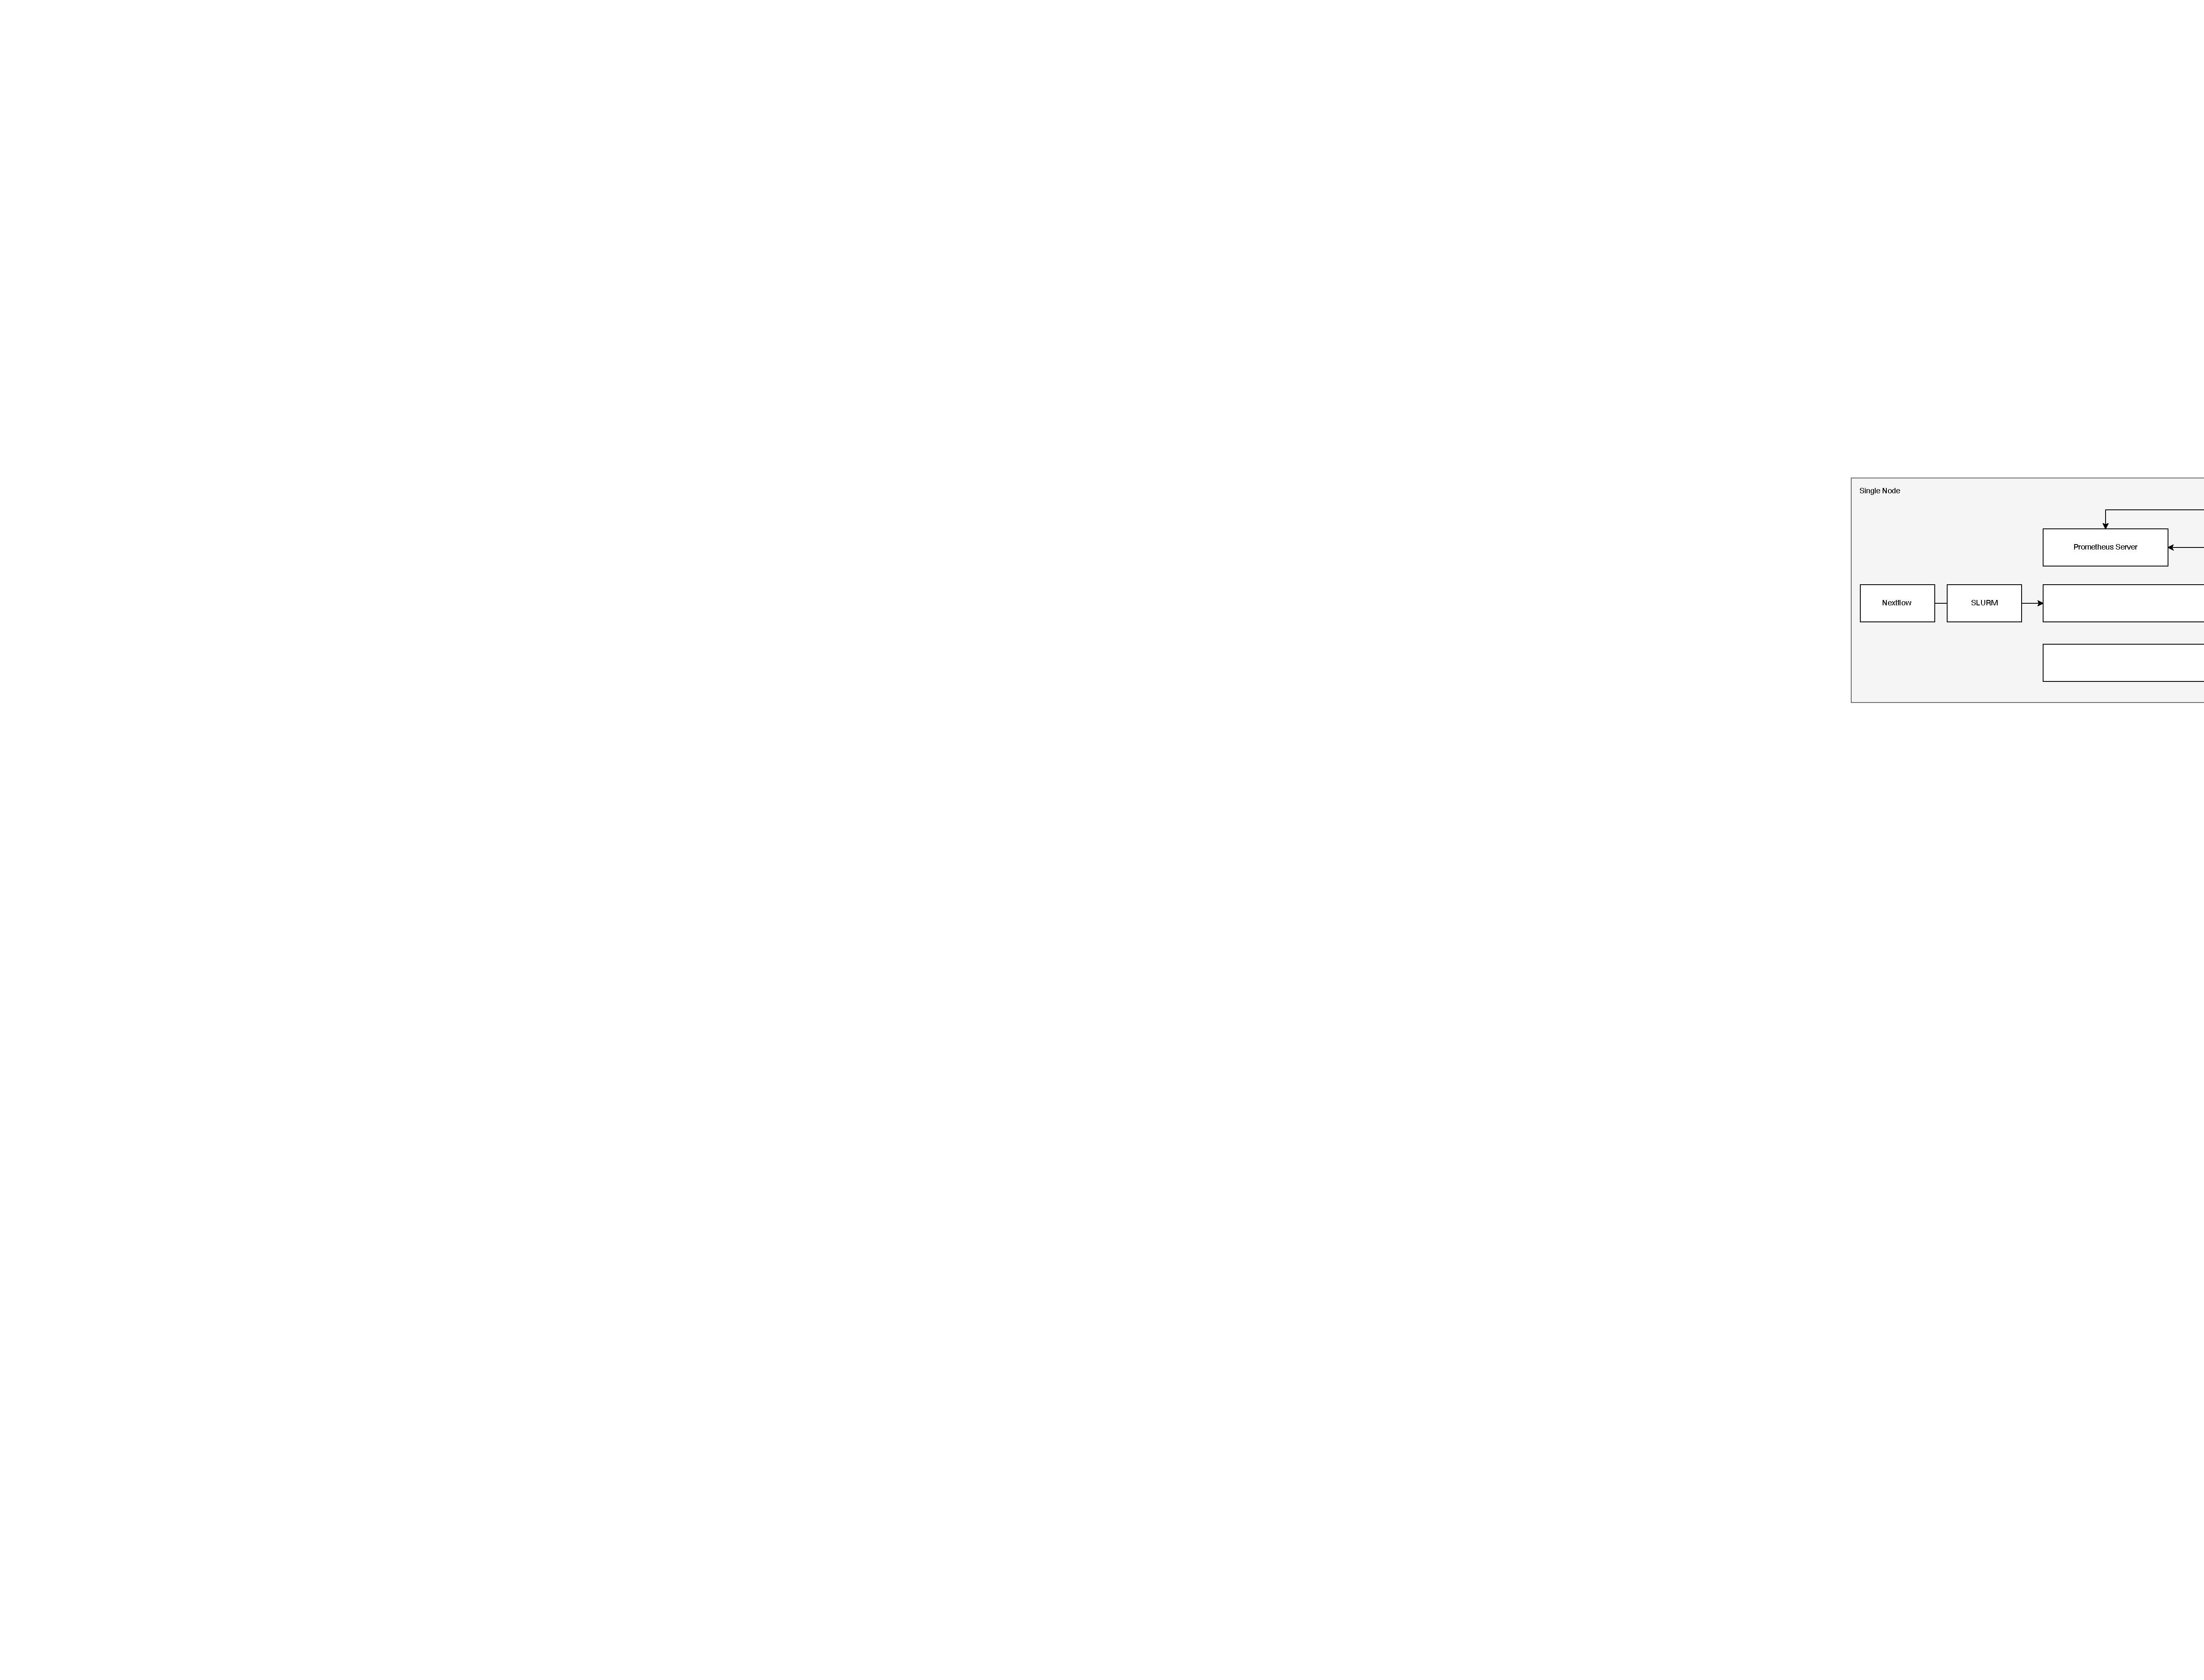
\includegraphics[width=\textwidth]{/home/nfomin3/dev/ThesisDocument/fig/04/04-monitoring.pdf} % Adjust the path if needed
    \caption{The monitoring client alongside the needed system components.}
    \label{fig:monitoring_client}
\end{figure}

The design of distributed HPC systems centers on three core aspects: resource allocation, queue ordering and dispatching, and job placement. In \ref{fig:monitoring_client } we adapt these core aspects and design a controller component that is responsible for invoking a central resource manager. The resource management component itself is steering the scheduling of tasks, the DAG-aware queue management, the assignment of tasks to the available compute nodes and eventually the allocation and execution on resources.
Since we aim to gain insight into the effectiveness of task co-location the processing engine of the simulator needs to offer an interface for alternative scheduling, task mapping and allocation strategies, ranging from conventional First-in-First-out (FIFO) ordering to heuristic reordering and placement that prioritizes beneficial pairings.

\subsubsection{Embedding Task Co-location into Scheduling Heuristics}
\label{sec:heuristic_design}

% Figure with Task Placement on VMs
\begin{figure}[htbp]
    \centering
    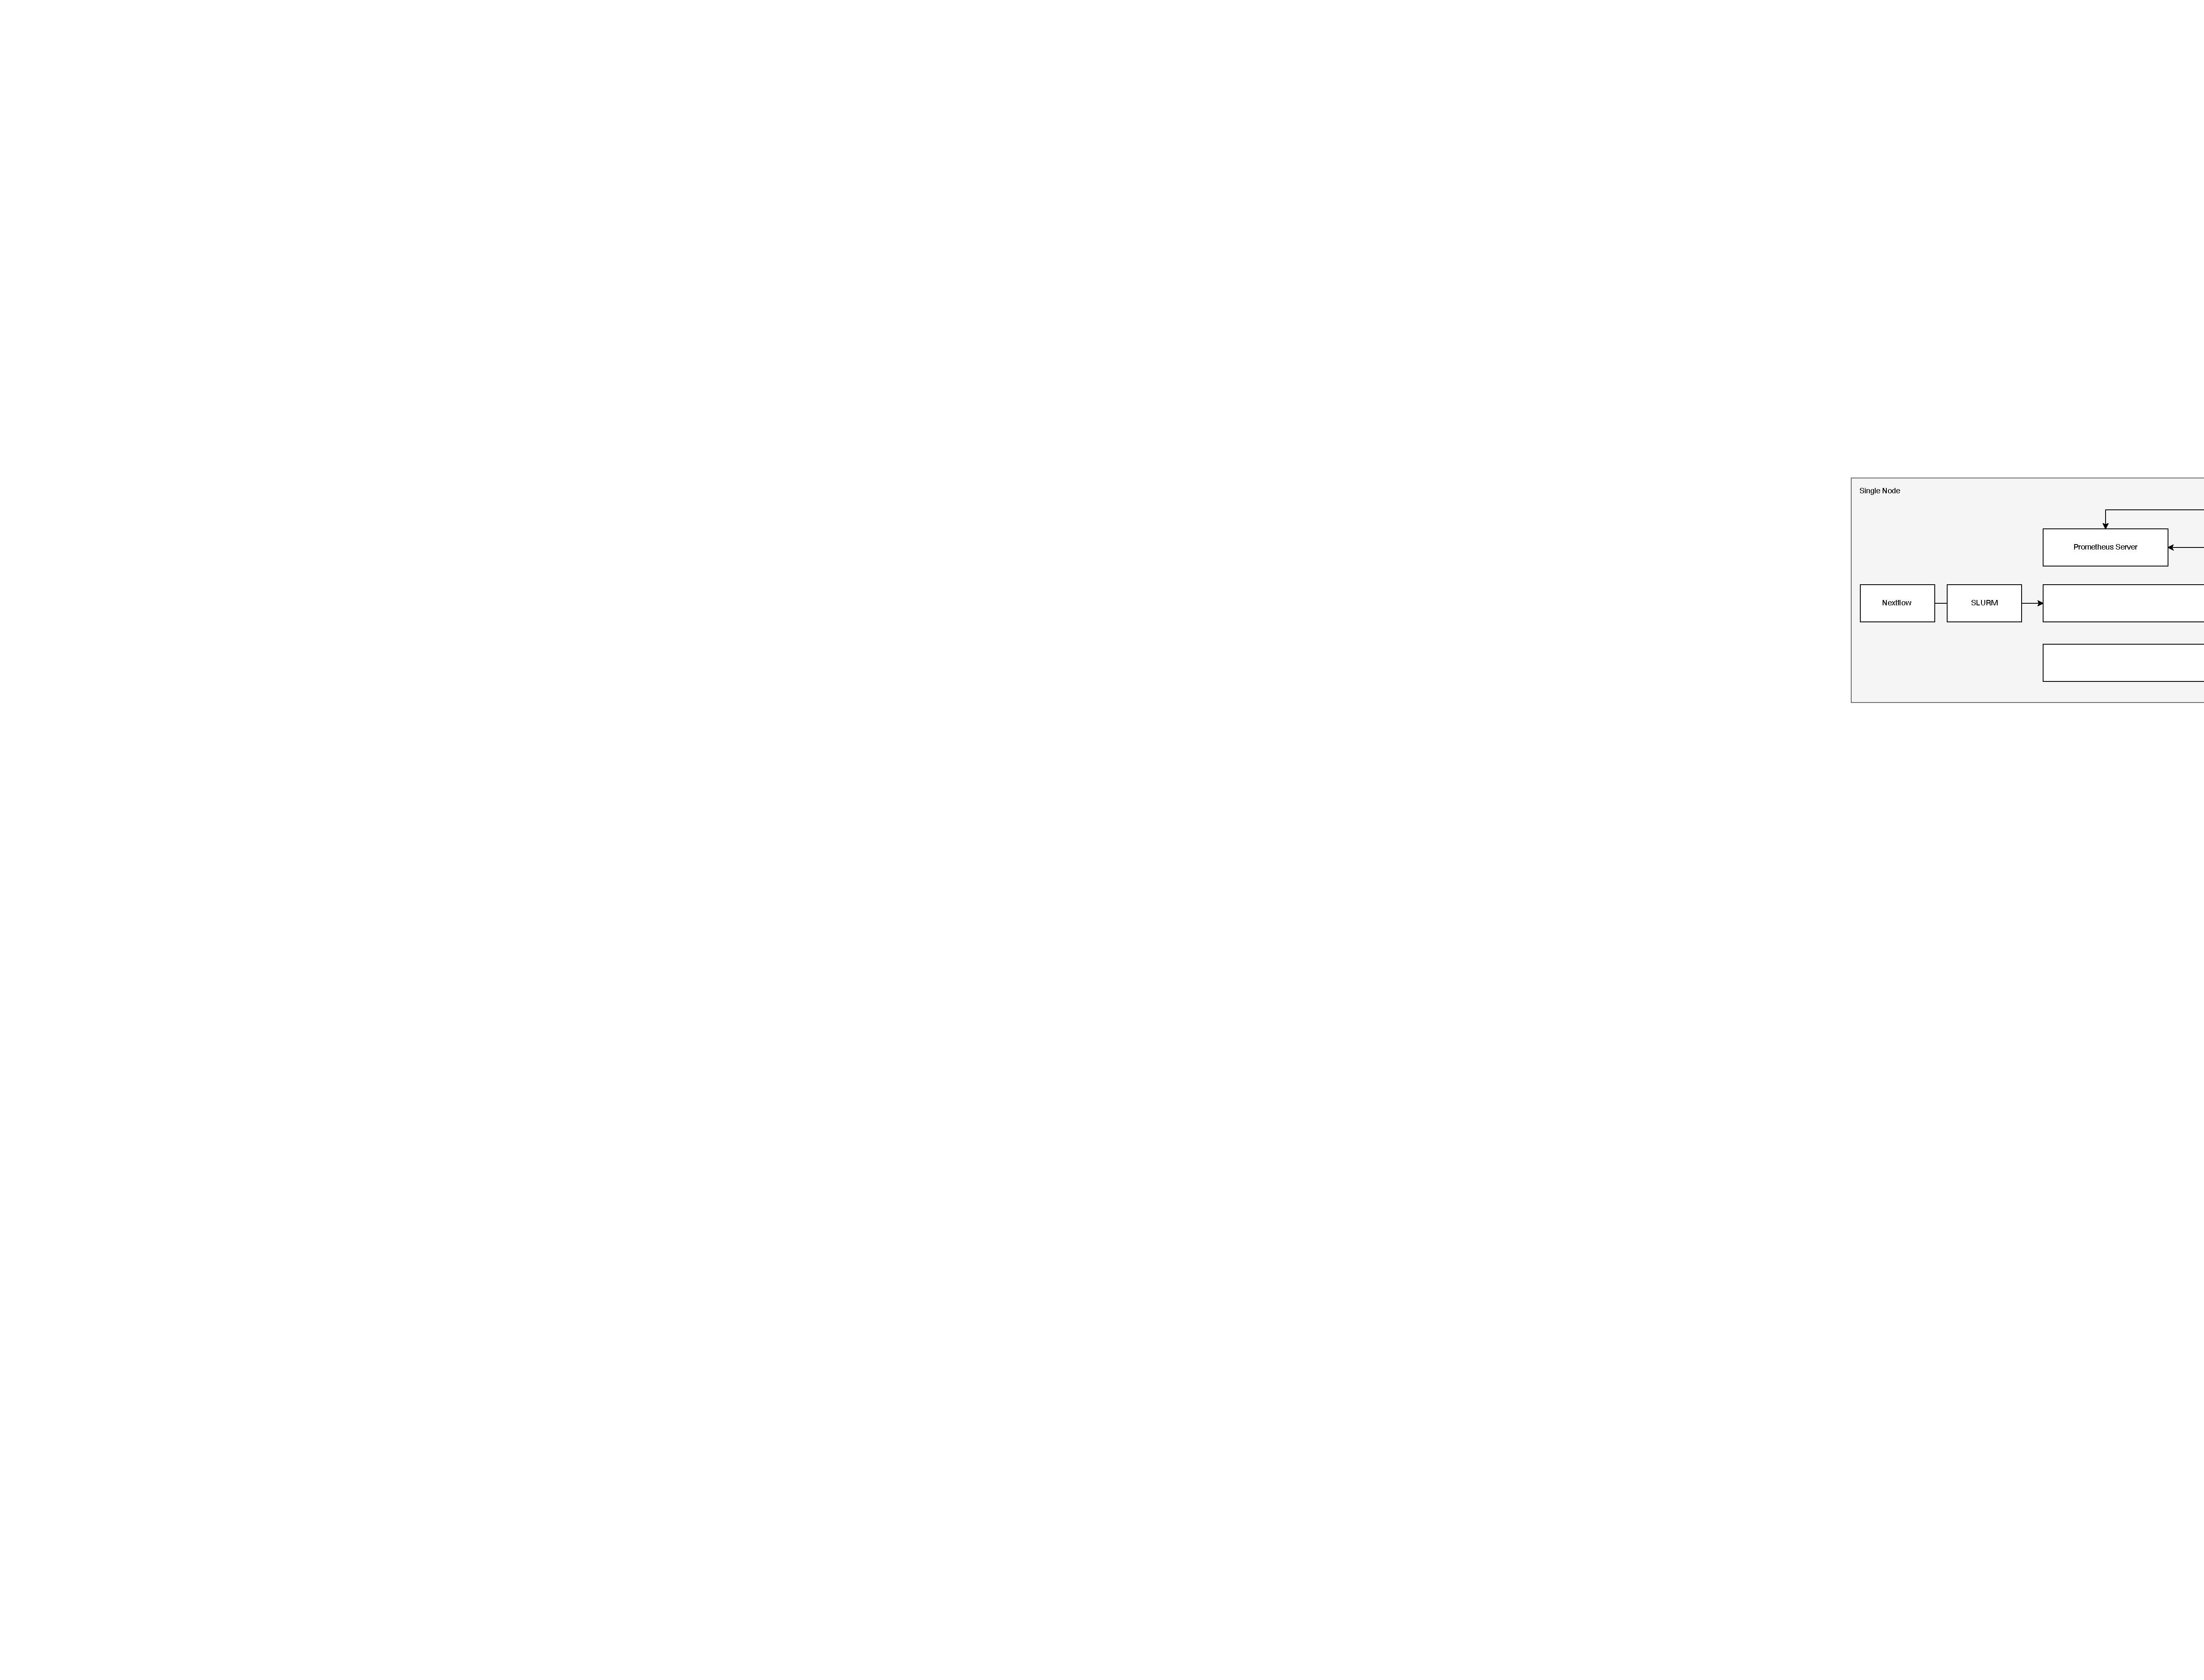
\includegraphics[width=\textwidth]{/home/nfomin3/dev/ThesisDocument/fig/04/04-monitoring.pdf} % Adjust the path if needed
    \caption{The monitoring client alongside the needed system components.}
    \label{fig:monitoring_client}
\end{figure}

Our algorithmic approach to define the behavior of the component's resource manager, allocator and scheduler introduced in \ref{fig:monitoring_client} is grounded in heuristic principles.
We choose to not formulate the embedding of co-location into the scheduling process as an optimization problem but through decision-making within simple, interpretable rules. Heuristic algorithms are well suited for such settings because they rely on deterministic, rule-based traversal of the search space rather than exhaustive or stochastic exploration.  We divide the task-to-node mapping into two steps. \ref{fig:monitoring_client} illustrates this approach.  The simulation launches the controller component which invokes our resource manager. Through the queue management the resource manager retrieves a set of ready-to-run tasks without predeccessors, that they depend on. In our example task 1,2,4,8,11,12,15 are to be scheduled. For the scheduling we choose to adpot list-scheduling algorithms, which form one of the most established heuristic approaches for workflow scheduling. They assign a priority or ranking to each task based on topological and performance factors (e.g., critical path length, execution cost, or communication overhead), producing a priority list. They then iteratively select the highest-priority unscheduled task and map it to a available resources. As we are interest in mapping not singel tasks but clusters of tasks we identify to embed the infomation retrieval on beneficial task consolidation at this exact stage during the scheduling process. The co-location hints my yield in consolidating T1, (T2, T4, T7), T8, (T11, T12) and T15. Lastly, we need to decide which host can accomodate the formed task clusters the best. We again define an interface for node assignment strategies either prioritize the host with the most idle compute cores first or tries to distribute the task clusters among all the available hosts in a fair manner. Finally the allocaiton component creates virtual machines that contain the task clusters and launch them on the assigned host. By this examplified design, we create a ground to not only embed and study the co-location problem in an execution environment but also gain the possibility of implementing different means of comparison through the interfaces per component. The next section formally introduce the simulation environment, consisting of the scientific workflow as the application that executes tasks and a system model that we use to represent our algorithmic approach to the co-location problem.

% System Model that was used for the heuristic design.
\paragraph{Simulation System Model}

\textbf{Workflow Properties}

Let the workflow be represented as a directed acyclic graph (DAG)
\[
    G = (T, E)
\]
where
\begin{itemize}
    \item $T = \{t_1, t_2, \dots, t_n\}$ denotes the set of \textbf{tasks}, and
    \item $E \subseteq T \times T$ denotes \textbf{data or control dependencies} between tasks.
\end{itemize}
A directed edge $(t_i, t_j) \in E$ indicates that task $t_j$ can start only after $t_i$ has completed.

\textbf{Task Properties}

Each task \( t_i \in T \) is associated with the following attributes:
\[
    \begin{array}{rcll}
        \text{req\_cores}(t_i) & \in & \mathbb{N}_{\ge 1} & \text{number of CPU cores required}, \\[4pt]
        \text{req\_mem}(t_i)   & \in & \mathbb{R}_{>0}    & \text{memory requirement in bytes.}
    \end{array}
\]

\textbf{Infrastructure Model}

Let \( \mathcal{H} = \{h_1, h_2, \dots, h_m\} \) denote the set of available \textbf{hosts},
where each host \( h_j \) is characterized by
\[
    C_j \in \mathbb{N}_{>0} \text{ (total number of cores)}, \qquad
    c(h_j) \in \mathbb{N}_{\ge 0} \text{ (current number of idle cores).}
\]

A \textbf{virtual machine (VM)} is represented as
\[
    v = (C_v, M_v, h_j),
\]
where \( C_v \) is the number of virtual cores, \( M_v \) the assigned memory,
and \( h_j \) the physical host on which it is instantiated.

The set of currently \textbf{ready tasks} (those whose dependencies are satisfied) is denoted by
\[
    \mathcal{Q} = \{t_1, t_2, \dots, t_k\}.
\]

\textbf{Resource Assignment}

A mapping of tasks to hosts and VMs is represented as
\[
    M = (h, \mathcal{T}_h, \text{colocMap}_h, \Phi_h),
\]
where
\begin{itemize}
    \item $h \in \mathcal{H}$ is the assigned host,
    \item $\mathcal{T}_h \subseteq T$ is the set of tasks mapped to $h$,
    \item $\text{colocMap}_h$ describes task clusters on $h$, and
    \item $\Phi_h$ represents associated file or data locations.
\end{itemize}
The set of mappings for an allocation interval is written as
\[
    \mathcal{M} = \{ M_1, M_2, \dots, M_p \}.
\]

\textbf{Task Co-location}

A \textbf{co-location mapping}, produced by a scheduler is defined as
\[
    \text{colocMap} = \{ (C_i, \mathcal{C}_i) \mid \mathcal{C}_i \subseteq T \},
\]
where $\mathcal{C}_i$ is a \textbf{cluster of tasks} to be executed together within a single virtual machine, ideally selected based on their resource affinity or complementary utilization patterns.

\textbf{Oversubscription}

An \textbf{oversubscription factor} $\alpha \in [0,1]$ allows up to
\[
    N_{\max}(h_j) = \lceil C_j (1 + \alpha) \rceil
\]
tasks to be scheduled concurrently on a VM on host $h_j$.


\textbf{Execution Dynamics}

At runtime:
\begin{itemize}
    \item \textbf{Node Assigners} determine host placement.
    \item \textbf{Schedulers} generate task queues and co-location groupings.
    \item \textbf{Allocators} instantiate and start VMs according to host-task mappings.
    \item The \textbf{Job Manager} executes tasks, monitors VM lifecycles, and updates resource states.
\end{itemize}

% TODO: Move to evaluation.
To evaluate the effectiveness of the proposed approach, we compare it against a series of progressively refined baseline algorithms that address the co-location problem with increasing complexity. These baselines range from simple scheduling heuristics to more advanced strategies that gradually incorporate awareness of co-location effects. The following table summarizes all baselines considered in this study. It is important to note that while some of them already involve concurrent execution of tasks, this represents uncontrolled co-location rather than informed or optimized placement. For clarity and conciseness, detailed algorithmic designs of these baselines are provided in the appendix, while this section focuses on describing their conceptual behavior.

Using the modelling introduced above, we construct an algorithm that depicts the overall behavior of our simulation approach.

% Blueprint Algorithm 

\begin{algorithm}[H]
    \caption{ShaReComp Simulation - WRENCH Framework}
    \label{alg:sharecomp_unified}
    \KwIn{workflow \( G=(T,E) \), hosts \( \mathcal{H}=\{h_1,\dots,h_m\} \), scheduling policy \( \pi \), oversubscription factor \( \alpha \), optional co-location API \( \mathcal{S} \)}
    \KwOut{workflow executed with policy-driven scheduling, node assignment, and adaptive resource management}

    \BlankLine
    Initialize system state: host capacities, ready queue \( \mathcal{Q} \), and monitoring layer\\

    \While{workflow \( G \) not completed}{
        Update \( \mathcal{Q} \) with all newly ready tasks\\
        Perform \textbf{task scheduling}: prioritize tasks in \( \mathcal{Q} \) according to policy \( \pi \)\\
        Perform \textbf{node assignment}: select suitable host(s) \( h \in \mathcal{H} \) using \( \pi \)\\
        Perform \textbf{resource allocation}: determine allowed capacity \( n_{\max}=f(c(h),\alpha) \) and reserve resources\\
        \If{policy \( \pi \) supports co-location}{
            Optionally query \( \mathcal{S} \) to group tasks by affinity and launch them on shared VMs
        }\Else{
            Launch one task per VM on assigned host
        }
        Monitor execution and task completions\\
        Release resources and enqueue successors of completed tasks
    }
    \Return{workflow complete}
\end{algorithm}

To compare the effectivness of using the ShaReComp approach we define multiple algorithms for the scheduling and node assignment phase that either employ exclusive resource assignment, assign tasks to multiple hosts in parallel or cluster random tasks into virtual machines. Generically all algorithms build on our simulation blueprint showed above \ref{alg:sharecomp_unified}. We call these algorithms baselines. In fact, we implement two baselines where each task gets executed in it's own VM, so no co-location is applied at all. Baselines 3, 3.1 and 3.2 co-locate tasks onto virtual machines and experiment with prioritizing the available compute hosts according to different strategies. Baselines 4 and 4.1 employ oversubscription, meaning that more tasks than reserved compute resources get assigned to a VM, strategically forcing resource contention. All baseline algorithms are included in the appendix of this thesis. In \ref{cha:evaluation} we include more detailed descriptions on the behavior and choice for the baseline algorithms.

\paragraph{Algorithmic Examples of Task Mapping with guided Co-location}
\label{sec:co-location_strategies}

This chapter on our approach concludes with introducing our main contribution of this thesis. We use our simulation framework to implement the ShaReComp approach directly into the workflow execution process. Therefore, we design four algorithms in 4 different versions of ShaRiff. ShaRiff is an acronym for share ressource if feasible. Each ShaRiff version implements a different strategy of mapping consolidated tasks onto availabel compute hosts while the decision maing for the co-location itself is always guided by the ShaReComp approach, introdcued in \ref{sec:task_clustering}.
Table \ref{tab:shariff_overview} provides an overview of the key differences between the ShaRiff algorithms.

% Table with ShaRiff Overview stuff.
\begin{table}[H]
    \centering
    \caption{Overview of ShaRiff and ShaReComp Scheduling Algorithms.}
    \label{tab:shariff_overview}
    \begin{tabularx}{\textwidth}{l l X}
        \toprule
        \textbf{Algorithm} & \textbf{Type}                                         & \textbf{Description}                                                                                                                         \\
        \midrule
        ShaRiff 1          & Contention-Aware Co-location                          & Uses the ShaReComp API to determine affinity-based co-location groups, minimizing interference between tasks.                                \\

        ShaRiff 2          & Adaptive Co-location + Over-Subscription              & Extends ShaRiff 1 by allowing safe CPU over-subscription based on affinity predictions.                                                      \\

        ShaRiff 3          & Round-Robin Node Assignment + Co-location             & Schedules tasks round-robin across hosts while applying affinity-based co-location through the ShaReComp API.                                \\

        ShaReComp          & Adaptive Max-Parallel Co-location + Over-Subscription & Integrates parallel scheduling, affinity-based co-location, and controlled over-subscription for optimized throughput and energy efficiency. \\
        \bottomrule
    \end{tabularx}
\end{table}

In the following we will in-depth describe the behavior of the ShaRiff algorithms one by one.

% ShaRiff 1

% Algorithm
\begin{algorithm}[H]
    \caption{ShaRiff 1 — Contention-aware Max-Parallel VM Co-Location Scheduling}
    \label{alg:sharecomp}
    \KwIn{workflow \( G=(T,E) \), hosts \( \mathcal{H}=\{h_1,\dots,h_m\} \), idle cores \( c(h_j) \), ShaReComp co-location API \( \mathcal{S} \)}
    \KwOut{all tasks \( t_i\in T \) executed with contention-aware co-location for improved efficiency and utilization}

    \BlankLine
    Initialize idle cores \( c(h_j)\gets C_j \) for all \( h_j\in\mathcal{H} \);
    Initialize ready queue \( \mathcal{Q} \) with all source tasks of \( G \) (FIFO order)

    \BlankLine
    \While{not all tasks \( t_i\in T \) completed}{
        \If{\( \mathcal{Q} \) is empty}{
            Wait until any task \( t_r \) completes;
            Release its cores: \( c(h(t_r)) \gets c(h(t_r)) + \text{req\_cores}(t_r) \);
            For each successor \( t_s \) of \( t_r \), enqueue \( t_s \) into \( \mathcal{Q} \) if all predecessors are completed;
            \textbf{continue}
        }

        Build available-host list \( L=\{\,h\in\mathcal{H}\mid c(h)>0\,\} \), sorted by \( c(h) \) descending;
        Initialize empty host task mapping list \( \mathcal{M} \);

        \BlankLine
        \ForEach{host \( h\in L \) and while \( \mathcal{Q} \) not empty}{
            Select up to \( c(h) \) ready tasks from \( \mathcal{Q} \) into \( \mathcal{T}_h \);
            Compute file-location map \( \Phi(\mathcal{T}_h) \);
            Query ShaReComp API: \( \text{colocMap} \gets \mathcal{S}(\mathcal{T}_h) \) \tcp*[r]{returns co-location groups}
            Add mapping \( (h,\mathcal{T}_h,\Phi(\mathcal{T}_h),\text{colocMap}) \) to \( \mathcal{M} \);
        }

        \BlankLine
        \ForEach{mapping \( (h,\mathcal{T}_h,\Phi,\text{colocMap}) \in \mathcal{M} \)}{
            \ForEach{group \( \mathcal{C}_k \in \text{colocMap} \)}{
                \( C_{\text{req}} \gets \text{sum(req\_cores}(\mathcal{C}_k)) \);
                \( M_{\text{req}} \gets \text{sum(req\_mem}(\mathcal{C}_k)) \);
                Allocate \( v_h = (C_{\text{req}}, M_{\text{req}}, h) \);
                Launch all \( t \in \mathcal{C}_k \) on \( v_h \);
                \( c(h) \gets \max(0, c(h) - C_{\text{req}}) \);
                Remove \( \mathcal{C}_k \) from \( \mathcal{Q} \);
            }
        }

        \BlankLine
        Wait until any task \( t_r \) completes;
        Release its cores: \( c(h(t_r)) \gets c(h(t_r)) + \text{req\_cores}(t_r) \);
        \If{no active tasks remain on its VM}{ Destroy VM }
        For each successor \( t_s \) of \( t_r \): if all predecessors are completed, enqueue \( t_s \) into \( \mathcal{Q} \);
    }
    \Return{workflow complete}

\end{algorithm}
This variant implements ShaRiff 1, which augments the FIFO pipeline with the external co-location adviser ShaReComp and a cluster-aware allocator. Tasks are dequeued in strict arrival order. Before placement, the scheduler invokes ShaReComp with the current set of ready tasks and receives clusters of jobs that are computed to co-locate well. The node-assignment stage then ranks hosts by descending idle-core capacity and fills the largest host first: it forms a batch of up to that hosts idle cores and attaches the ShaRiff cluster map to the batch; if tasks remain, it proceeds to the next host in the ranked list. A small-queue fast path ensures dispatch even when only a few tasks are available.
The allocator realizes the advisers plan one VM per recommended cluster on the chosen host. For each multi-task cluster, it provisions a VM whose vCPU count and memory equal the sum of the clustered tasks declared requirements, starts the VM, and submits the tasks to that same virtual compute service. Singleton clusters are grouped into a shared VM on the host to avoid VM fragmentation; each submitted task keeps its own job identity, and the allocator tracks VM lifecycle across all tasks assigned to it, tearing the VM down only after the last co-located task completes.
Conceptually, ShaRiff preserves FIFO ordering and capacity-ranked host filling, but replaces random batching with adviser-driven clustering. The effect is to co-locate tasks that are likely complementary, thereby reducing contention and improving per-host utilization without oversubscription. When the adviser yields single tasks, the system still shares if feasible by pooling them into a shared VM, maintaining the same deterministic provisioning and lifecycle rules.

% ShaRiff 2

% Algorithm
\begin{algorithm}[H]
    \caption{ShaRiff 2 — Adaptive Max-Parallel VM Co-Location with Controlled Over-Subscription}
    \label{alg:sharecomp_oversub}
    \KwIn{workflow \( G=(T,E) \), hosts \( \mathcal{H}=\{h_1,\dots,h_m\} \), idle cores \( c(h_j) \), oversubscription factor \( \alpha \), ShaReComp co-location API \( \mathcal{S} \)}
    \KwOut{workflow executed with affinity-based co-location, maximal host parallelism, and safe oversubscription}

    \BlankLine
    Initialize idle cores \( c(h_j)\gets C_j \) for all \( h_j\in\mathcal{H} \)
    Initialize ready queue \( \mathcal{Q} \) with all source tasks of \( G \) (FIFO order)

    \BlankLine
    \While{not all tasks \( t_i\in T \) completed}{
        \If{\( \mathcal{Q} \) is empty}{
            Wait until any task \( t_r \) completes
            Release its cores: \( c(h(t_r)) \gets c(h(t_r)) + \text{req\_cores}(t_r) \)
            For each successor \( t_s \) of \( t_r \), enqueue \( t_s \) into \( \mathcal{Q} \) if all predecessors are completed\\
            \textbf{continue}
        }

        Build available-host list \( L=\{\,h\in\mathcal{H}\mid c(h)>0\,\} \), sorted by \( c(h) \) descending
        Initialize empty host task mapping list \( \mathcal{M} \)

        \BlankLine
        \ForEach{host \( h\in L \) and while \( \mathcal{Q} \) not empty}{
            Compute oversubscription limit \( n_{\max} = \lceil c(h) \times (1 + \alpha) \rceil \)
            Select up to \( n_{\max} \) ready tasks from \( \mathcal{Q} \) into \( \mathcal{T}_h \)
            Compute file-location map \( \Phi(\mathcal{T}_h) \)
            Query ShaReComp API: \( \text{colocMap} \gets \mathcal{S}(\mathcal{T}_h) \) \tcp*[r]{returns co-location groups}
            Add mapping \( (h,\mathcal{T}_h,\Phi(\mathcal{T}_h),\text{colocMap}) \) to \( \mathcal{M} \)
        }

        \BlankLine
        \ForEach{mapping \( (h,\mathcal{T}_h,\Phi,\text{colocMap}) \in \mathcal{M} \)}{
            \ForEach{group \( \mathcal{C}_k \in \text{colocMap} \)}{
                \( C_{\text{req}} \gets \text{sum(req\_cores}(\mathcal{C}_k)) \)
                \( M_{\text{req}} \gets \text{sum(req\_mem}(\mathcal{C}_k)) \)
                \If{\( C_{\text{req}} > c(h) \)}{
                    Allocate \( v_h = (c(h), M_{\text{req}}, h) \); \tcp*[r]{oversubscription active}
                }
                \Else{
                    Allocate \( v_h = (C_{\text{req}}, M_{\text{req}}, h) \)
                }
                Launch all \( t \in \mathcal{C}_k \) on \( v_h \)
                \( c(h) \gets \max(0, c(h) - C_{\text{req}}) \)
                Remove \( \mathcal{C}_k \) from \( \mathcal{Q} \)
            }
        }

        \BlankLine
        Wait until any task \( t_r \) completes
        Release its cores: \( c(h(t_r)) \gets c(h(t_r)) + \text{req\_cores}(t_r) \)
        \If{no active tasks remain on its VM}{ Destroy VM }
        For each successor \( t_s \) of \( t_r \): if all predecessors are completed, enqueue \( t_s \) into \( \mathcal{Q} \)
    }
    \Return{workflow complete}
\end{algorithm}

% ShaRiff 2
This variant retains the ShaRiff-augmented FIFO pipeline but enables controlled oversubscription during placement and VM sizing. Tasks are dequeued in arrival order. Before dispatch, the scheduler queries ShaReComp with the current ready set and receives clusters of tasks pcomputed to co-locate well. Hosts are ranked by descending idle-core capacity; the assigner then fills the largest host first with a batch whose size may exceed the hosts free cores by a fixed factor of in our example 25\%. If tasks remain, it proceeds to the next host and repeats.
The allocator implements the advisers plan one VM per cluster on the chosen host, but with oversubscription semantics. For multi-task clusters, it provisions a VM whose vCPU and memory equal the sum of the clusters requests—even if that exceeds the hosts currently free cores. For single task clusters collected on the same host, it provisions a shared VM and caps vCPUs at the hosts free cores when necessary. In both cases the VM is started once, all tasks in the cluster are submitted to the same virtual compute service, and the VM is torn down only after the last co-located task finishes.
Because ShaReComp groups complementary tasks, oversubscription holds the potential to translate into higher throughput and energy efficiency. However, when clustered tasks are less complementary, contention can surface, making this variant an explicit trade-off between utilization and interference.

% ShaRiff 3

% Algorithm

\begin{algorithm}[H]
    \caption{ShaRiff 3 — Round-Robin Node Assignment with contention-aware VM Co-Location}
    \label{alg:sharecomp_rr}
    \KwIn{workflow \( G=(T,E) \), hosts \( \mathcal{H}=\{h_1,\dots,h_m\} \), idle cores \( c(h_j) \), ShaReComp co-location API \( \mathcal{S} \)}
    \KwOut{tasks executed using round-robin host selection with affinity-based VM co-location}

    \BlankLine
    Initialize idle cores \( c(h_j)\gets C_j \) for all \( h_j\in\mathcal{H} \)
    Initialize ready queue \( \mathcal{Q} \) with all source tasks of \( G \) (FIFO order)
    Initialize round-robin index \( r \gets 0 \)

    \BlankLine
    \While{not all tasks \( t_i\in T \) completed}{
        \If{\( \mathcal{Q} \) is empty}{
            Wait until any task \( t_r \) completes
            Release its cores: \( c(h(t_r)) \gets c(h(t_r)) + \text{req\_cores}(t_r) \)
            For each successor \( t_s \) of \( t_r \), enqueue \( t_s \) into \( \mathcal{Q} \) if all predecessors are completed\\
            \textbf{continue}
        }

        Select next host \( h = \mathcal{H}[r \bmod |\mathcal{H}|] \)
        Update round-robin index: \( r \gets (r + 1) \bmod |\mathcal{H}| \)
        Retrieve available cores \( C = c(h) \)
        Select up to \( C \) ready tasks from \( \mathcal{Q} \) into \( \mathcal{T}_h \)
        Query ShaReComp API: \( \text{colocMap} \gets \mathcal{S}(\mathcal{T}_h) \) \tcp*[r]{returns co-location groups}

        \BlankLine
        \ForEach{group \( \mathcal{C}_k \in \text{colocMap} \)}{
            \( C_{\text{req}} \gets \text{sum(req\_cores}(\mathcal{C}_k)) \)
            \( M_{\text{req}} \gets \text{sum(req\_mem}(\mathcal{C}_k)) \)
            Allocate \( v_h = (C_{\text{req}}, M_{\text{req}}, h) \)
            Launch all \( t \in \mathcal{C}_k \) on \( v_h \)
            \( c(h) \gets \max(0, c(h) - C_{\text{req}}) \)
            Remove \( \mathcal{C}_k \) from \( \mathcal{Q} \)
        }

        \BlankLine
        Wait until any task \( t_r \) completes
        Release its cores: \( c(h(t_r)) \gets c(h(t_r)) + \text{req\_cores}(t_r) \)
        \If{no active tasks remain on its VM}{ Destroy VM }
        For each successor \( t_s \) of \( t_r \): if all predecessors are completed, enqueue \( t_s \) into \( \mathcal{Q} \)
    }
    \Return{workflow complete}
\end{algorithm}

ShaRiff 3 preserves FIFO dequeuing but combines round-robin first-fit placement with ShaReComp-guided intra-VM co-location. The scheduler releases tasks strictly in arrival order. The node-assignment component scans hosts in round-robin/first-fit fashion and picks the first host reporting at least one idle core. It then pulls up to that hosts idle-core capacity worth of ready tasks and queries ShaReComp for a co-location plan over this batch.
The allocator realizes ShaReComps plan one VM per suggested cluster on the chosen host. For each multi-task cluster, it sizes the VM by summing vCPU and memory requirements of the clusters tasks, starts the VM, and submits all cluster tasks to the same virtual compute service. Tasks that ShaReComp leaves as singletons are grouped onto an additional shared VM on that host; its size is the aggregate of the singletons requests.
Conceptually, the policy is first-fit host, adviser-driven packing. Unlike the max-parallel variants, this strategy does not oversubscribe cores. Tt fills only the currently free capacity of the first eligible host and relies on ShaReComp's clustering to raise utilization and efficiency through informed co-location.

% TODO: This part needs to be reworked.
% MinMin extension
This scheduler extension augments the ShaRiff-based variants with a MinMin ordering layer, a classical heuristic from list scheduling. In standard list scheduling, tasks are iteratively selected based on their earliest estimated completion time; Min Min specifically chooses, at each step, the task (or cluster) with the minimum predicted runtime among all ready candidates and schedules it first. Here, this principle is applied not to individual tasks but to task clusters produced by ShaRiffs co-location analysis.
For each scheduling interval, the scheduler requests from ShaRiff a co-location partition of the ready tasks, grouping them into clusters that are predicted to interact efficiently when sharing a VM. It then queries a prediction service for each cluster, obtaining runtime estimates through the chosen model (e.g., KCCA). The clusters are ordered by ascending predicted runtime, and this order defines the execution sequence. Node selection and VM provisioning are delegated to the ShaRiff node assignment and allocator components, which handle placement and resource sizing as usual.
Conceptually, this forms a Min Min list scheduler over co-located clusters: it maintains ShaRiffs intelligent co-location strategy while globally minimizing queueing delay and improving average completion time by prioritizing faster clusters. This layer is independent of the underlying allocation or node assignment logic and purely refines execution ordering to exploit performance prediction while preserving all structural and capacity constraints of the ShaRiff framework.